%\documentclass{book}\usepackage{sjtfonts}\usepackage{includegraphics}\usepackage{alltt}\usepackage{latexsym}
%\usepackage{array}
%\begin{document}\input{defs0}%		miradefs.tex 		    June 1994

% opening and closing a quoted Miranda section

\newcommand{\mira}{\noindent\hrulefill\nopagebreak\so}
\newcommand{\arim}{\nopagebreak\st\hrulefill\\}

% backslash in the Miranda environment
% Only feasible approach is to use \verb+\+
% in line!

%\newcommand{\bs}{$\mi\backslash\!\!$}
%\newcommand{\lbs}{\mbox{\verb+\+}}

% ignoring part of the input

\newcommand{\ignore}[1]{}

% a blank line in a Miranda section

\newcommand{\bl}{\mbox{\ }}

% Signalling a diffculty.

\definecolor{light-gray}{gray}{0.95}

\newcommand{\beware}[2]
 {\medskip\noindent\colorbox{light-gray}{\parbox{\textwidth}
 {\mbox{\large\textbf{#1}} \medskip\noindent\\ #2}\medskip\noindent}}

% Subscripting in Miranda text
\newcommand{\subscr}[2]{\mbox{${\mbox{\texttt{#1}}}_{\mbox{\texttt{#2}}}$}}

%\newcommand{\subscr}[2]{\mbox{${\mbox{\mi #1}}_{\mbox{\smtt #2}}$}}
\newcommand{\aone}{\subscr{a}{1}}
\newcommand{\atwo}{\subscr{a}{2}}
\newcommand{\ak}{\subscr{a}{k}}

\newcommand{\aoneone}{\subscr{a}{1,1}}

\newcommand{\eone}{\subscr{e}{1}}
\newcommand{\etwo}{\subscr{e}{2}}
\newcommand{\ei}{\subscr{e}{i}}
\newcommand{\er}{\subscr{e}{r}}

\newcommand{\fone}{\subscr{f}{1}}
\newcommand{\fl}{\subscr{f}{l}}

\newcommand{\gone}{\subscr{g}{1}}
\newcommand{\gtwo}{\subscr{g}{2}}
\newcommand{\gi}{\subscr{g}{i}}
\newcommand{\gr}{\subscr{g}{r}}

\newcommand{\hone}{\subscr{h}{1}}
\newcommand{\hl}{\subscr{h}{l}}

\newcommand{\pone}{\subscr{p}{1}}
\newcommand{\ptwo}{\subscr{p}{2}}
\newcommand{\pk}{\subscr{p}{k}}

\newcommand{\qone}{\subscr{q}{1}}
\newcommand{\qtwo}{\subscr{q}{2}}
\newcommand{\qk}{\subscr{q}{k}}

\newcommand{\rone}{\subscr{r}{1}}
\newcommand{\rtwo}{\subscr{r}{2}}

\newcommand{\tone}{\subscr{t}{1}}
\newcommand{\ttwo}{\subscr{t}{2}}
\newcommand{\tn}{\subscr{t}{n}}

\newcommand{\vone}{\subscr{v}{1}}
\newcommand{\vtwo}{\subscr{v}{2}}
\newcommand{\vn}{\subscr{v}{n}}

% for regular expressions

\newcommand{\stone}{\subscr{st}{1}}
\newcommand{\sttwo}{\subscr{st}{2}}
\newcommand{\stn}{\subscr{st}{n}}
\newcommand{\rthree}{\subscr{r}{3}}

\newcommand{\eps}{$\varepsilon$}
\newcommand{\trans}[1]{\stackrel{\mbox{\tt #1}}{\longrightarrow}}



% superscript in Miranda text

\newcommand{\superscr}[2]{\mbox{${\mbox{\mi #1}}^{\mbox{\smtt #2}}$}}

% Not equals in Miranda text

\newcommand{\noteq}{\makebox[0pt][l]{=}/}
\newcommand{\overslash}{\makebox[0pt][l]{/}}

% Definitions in complexity chapter

\newfont{\oldSym}{cmsy10}
\newcommand{\Th}{\boldmath$\oldSym\Theta$}
\newcommand{\pow}[1]{\^{}#1}
\newcommand{\leqq}{$\leq$}
\newcommand{\geqq}{$\geq$}
\newcommand{\lll}{$\ll$}
\newcommand{\eqq}{$\equiv$}
\newcommand{\ltwo}{\subscr{log}{2}}

% Indexing

\newcommand{\minx}[1]{\index{#1@{\ttfamily{}#1}}}
\setcounter{chapter}{13}\setcounter{page}{231}

\chapter{Algebraic types}
\chapstart
\label{algTypes}
\index{algebraic type|(}

\begin{figure}[t]
\begin{center}
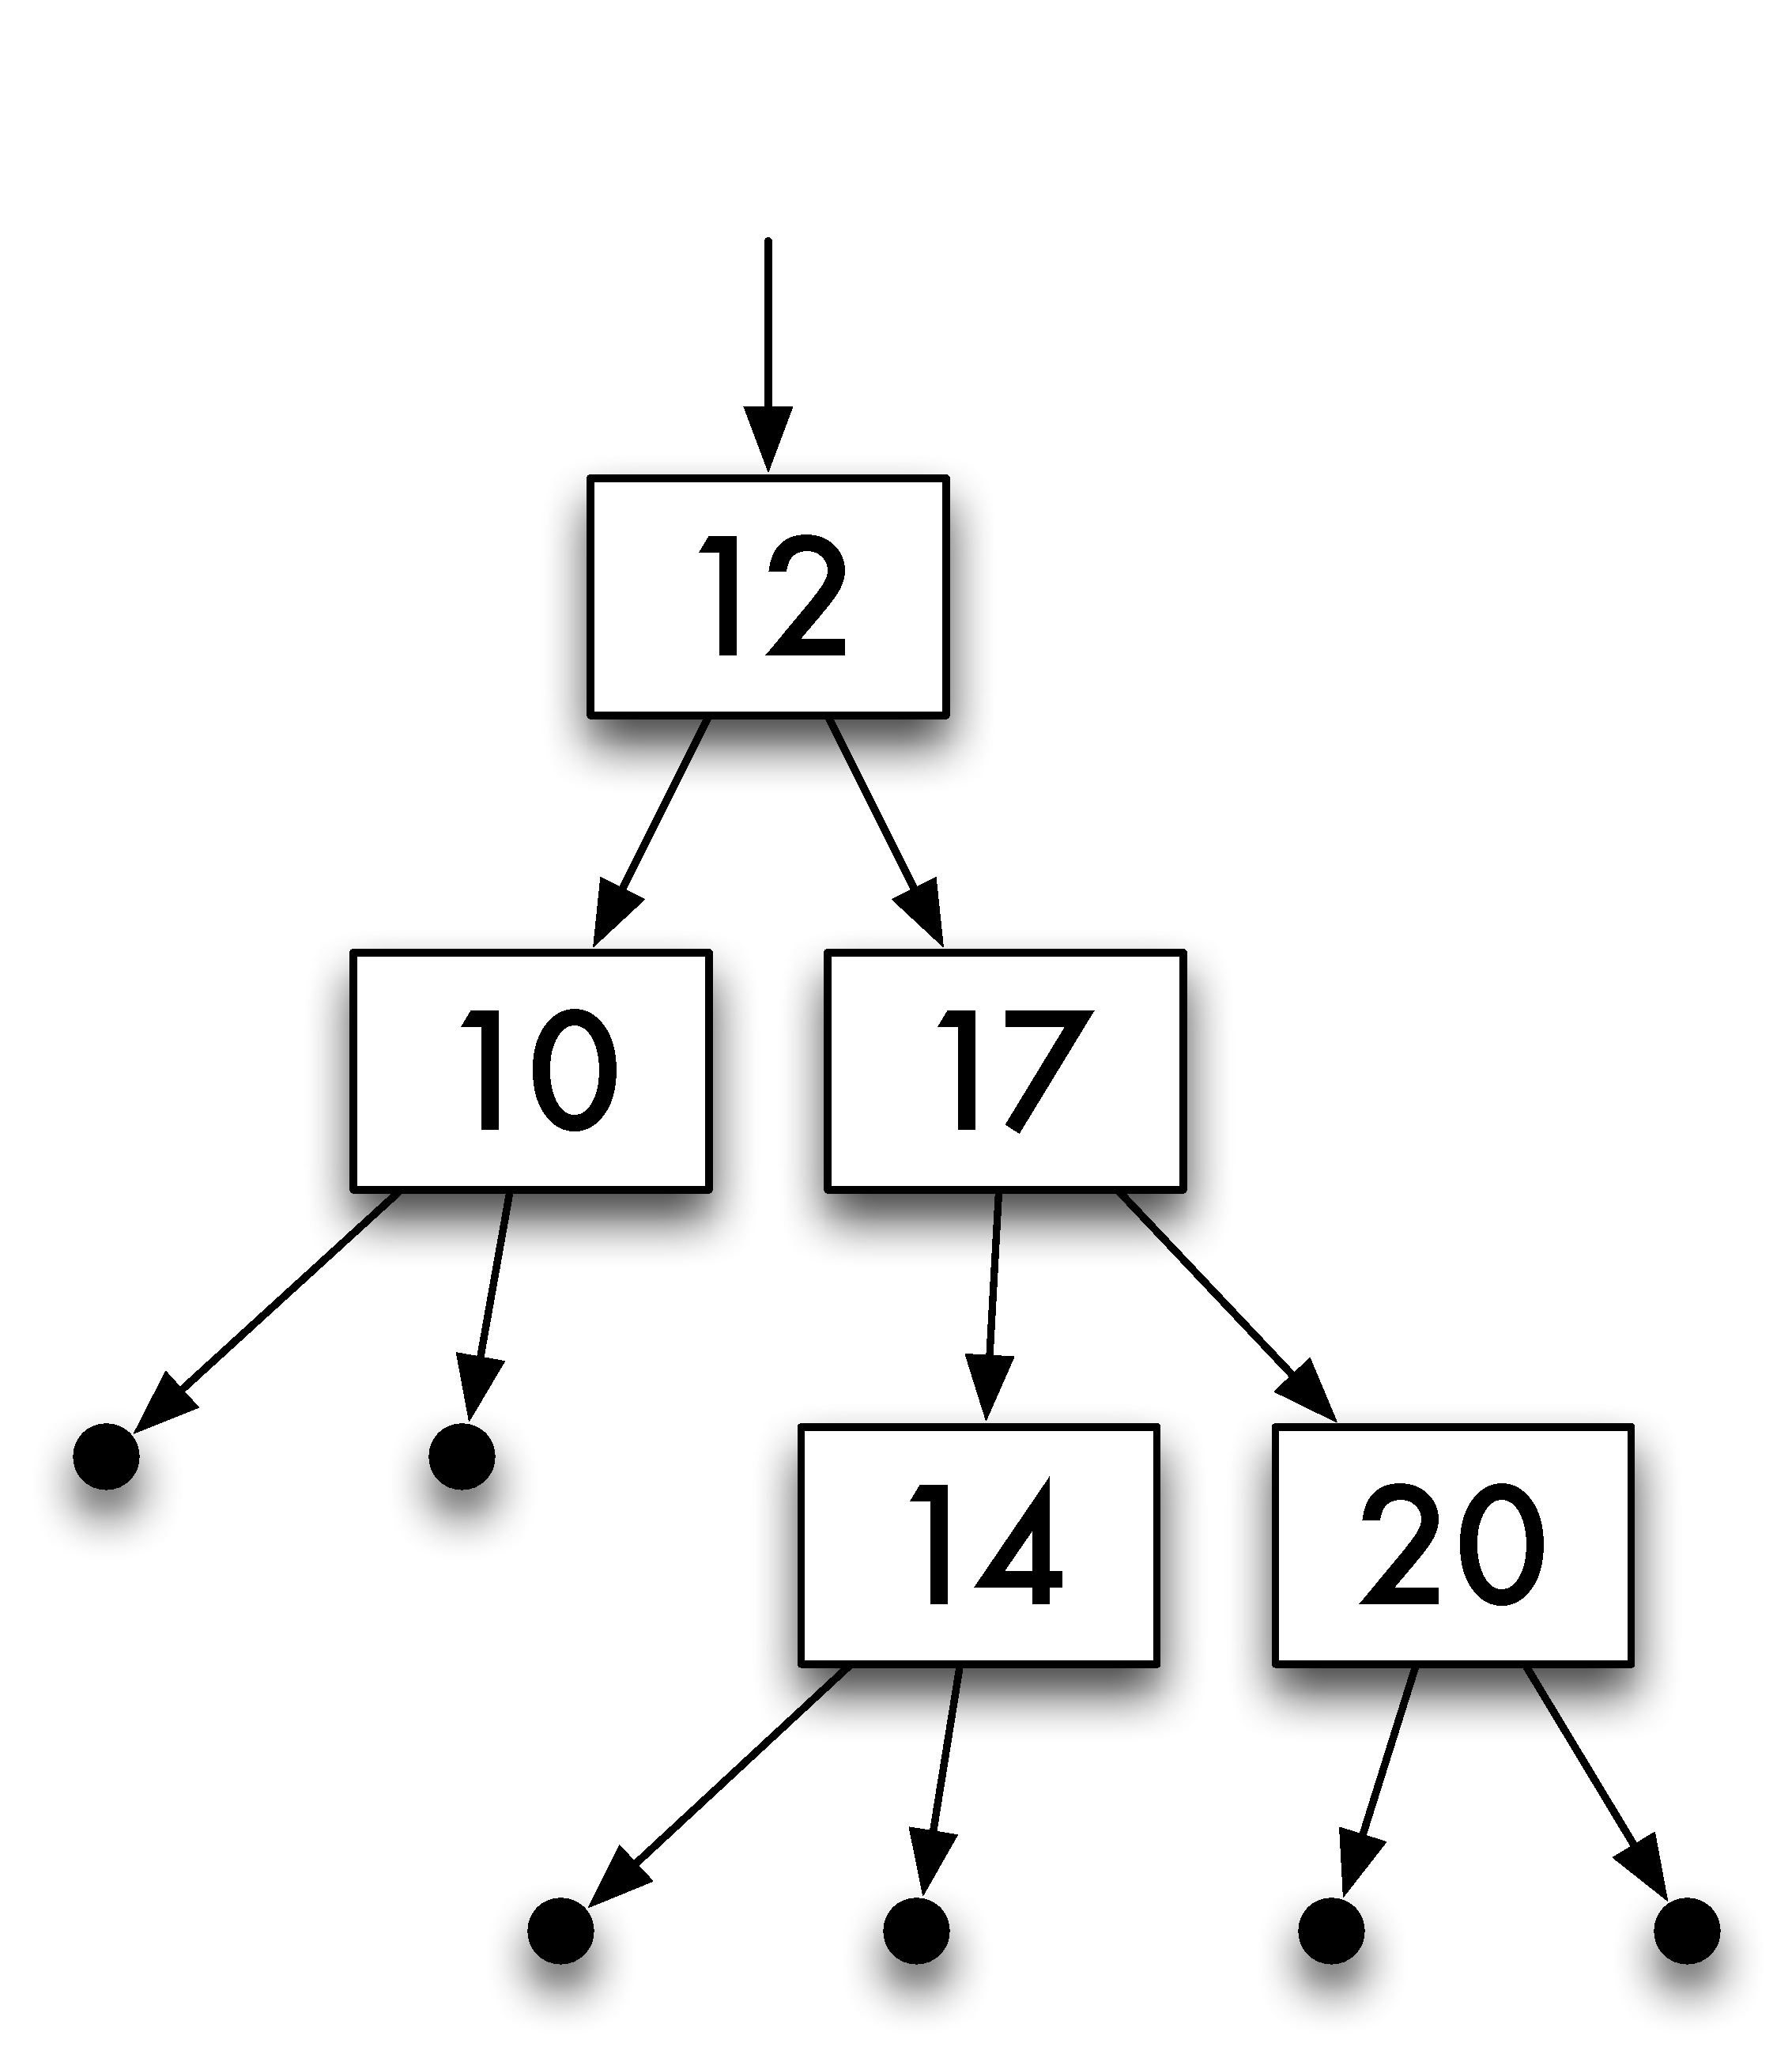
\includegraphics[width=3in]{Pictures/NewTree.pdf}
\end{center}
\caption{An example of a tree of integers.}
\label{treeFig}
\end{figure}

So far in our discussion of Haskell we have been able to model entities using
\begin{titemize}
\item the base types, \texttt{Int}, \texttt{Float}, \texttt{Bool} and \texttt{Char}, and
\item composite types: tuple types, \texttt{(\tone,\ttwo,\ldots,\subscr{t}{n})};
list types,
\texttt{[\tone]}; and function types, \texttt{(\tone\ -> \ttwo)}; where 
\texttt{\tone}, \ldots, \texttt{\subscr{t}{n}} are themselves types,
\item algebraic types, including enumerated types, as introduced in Section \ref{EnumTypes}, and product and sum type, first given in Section \ref{introAlg}.
\end{titemize}
This gives a wide range of types to use in modelling different domains in Haskell. This chapter completes our coverage of the topic of algebraic types and looks at two extensions in some detail:

\begin{titemize}
\item The types can be \textbf{recursive}\index{algebraic type!recursive|see{recursive type}};
we can use the type we are defining,
\texttt{Typename}, as (part of) any of the component types, as in the definition of numeric trees ``\texttt{NTree}s'':
\begin{alltt}
data NTree = NilT |\minx{NTree}
             Node Integer NTree NTree
\end{alltt}
an illustration of a tree from \texttt{NTree} is given in Figure \ref{treeFig}. Recursion in \texttt{data} type definitions gives us
lists, trees and many other useful data structures.
\item The name of the type being defined can be followed by one or more type
variables which may be used on the right-hand side, making the definition
\textbf{polymorphic}.\index{algebraic type!polymorphic} An example built-into Haskell is the \texttt{Maybe} type,
\begin{alltt}
data Maybe a = Nothing | Just a
\end{alltt}
which can be used in modelling program errors.
\end{titemize}
Recursive polymorphic types combine these two ideas, and this powerful
mixture provides types which can be reused in many different situations --
the built-in type of lists is an example which we have already seen. We'll look again at the \texttt{NTree} and \texttt{Maybe} types later in this chapter, and other
examples are given in the sections which follow.

\section{Algebraic type definitions revisited}
\label{algRevisited}
Algebraic data type definitions are introduced by the keyword \texttt{data}, followed by
\index{data@\texttt{data} type|see{algebraic type}}
the name of the type, an equals sign and then the
\textbf{constructors} of the\index{constructor}
type being defined.  The name of the type and the names of
constructors begin with
capital letters.

The general form of the algebraic type definitions which we have seen so far is \index{algebraic type!general form of definition}
\begin{alltt}
data Typename \hfill (Typename)
  = \subscr{Con}{1} \subscr{t}{11} \ldots \subscr{t}{1\subscr{k}{1}} | 
    \subscr{Con}{2} \subscr{t}{21} \ldots \subscr{t}{2\subscr{k}{2}} | 
        ....
    \subscr{Con}{n} \subscr{t}{n1} \ldots \subscr{t}{n\subscr{k}{n}}   
\end{alltt}
Each \texttt{\subscr{Con}{i}} is a constructor, followed by 
\subscr{k}{i}\ types, where \subscr{k}{i}\ is a non-negative integer which may
be zero. We build elements of the type \texttt{Typename} by applying these constructor
functions to arguments of the types given in the definition, so that
\begin{alltt}
\subscr{Con}{i} \subscr{v}{i1} \ldots \subscr{v}{i\subscr{k}{i}}
\end{alltt}
will be a member of the type \texttt{Typename} if \subscr{v}{ij} is 
in \subscr{t}{ij} for \texttt{j} ranging from \texttt{1} to \subscr{k}{i}. 
Reading the constructors as functions, the 
definition \texttt{(Typename)} gives the constructors the following
types
\begin{alltt}
\subscr{Con}{i} :: \subscr{t}{i1} -> \ldots -> \subscr{t}{i\subscr{k}{i}} -> Typename
\end{alltt}
Of the examples we have seen so far, enumerated types have constructors which take no arguments, 
\begin{alltt}
data Season = Spring | Summer | Autumn | Winter\minx{Season}
\end{alltt}
product types have a single constructor, 
\begin{alltt}
data People = Person Name Age \minx{People}
\end{alltt}
and sum types are the most general: they have a number of constructors taking different arguments, as in the definition
\begin{alltt}\minx{Shape}
data Shape = Circle Float |
             Rectangle Float Float
\end{alltt}
Definitions over algebraic types use pattern matching both to distinguish between different alternatives and to extract components from particular elements:
\begin{alltt}
area :: Shape -> Float
area (Circle r)      = pi*r*r
area (Rectangle h w) = h*w
\end{alltt}
As we discussed in Section \ref{haskellClasses},  Haskell has a number of built-in classes including
 \texttt{Eq},  \texttt{Ord}, 
  \texttt{Enum}, \texttt{Show}, and \texttt{Read}. When we introduce a new algebraic type it's possible to \texttt{derive} instances of these classes for the new type, like this:
\begin{alltt}\minx{Season}
data Season = Spring | Summer | Autumn | Winter 
              deriving (Eq,Ord,Enum,Show,Read)
\end{alltt}
We can thus compare seasons for equality and order, write expressions of
the form \texttt{[Spring .. Autumn]} denoting the list \texttt{[Spring, Summer, Autumn]}, and \texttt{show} and read values of the type.


\begin{exercises}





\item
Reimplement the library database\index{library database}
of Section \ref{library} to use an
algebraic type like \texttt{People} rather than a pair. Compare
the two approaches to this example.

\item
The library database of Section \ref{library} is to be extended in the
following ways.
\begin{titemize}
\item CDs and videos as well as books are available for loan.
\item A record is kept of the authors of books as well as their titles.
Similar information is kept about CDs, but not about videos.
\item Each loan has a period: books one month, CDs one week and videos three
days.
\end{titemize}
Explain how you would modify the types used to implement the database, and
how the function types might be changed. 
The system should perform the following operations. For each case, give the
types and definitions of the functions involved.
\begin{titemize}
\item Find all items on loan to a given person.
\item Find all books, CDs or videos on loan to a particular person.
\item Find all items in the database due back on or before a particular day,
and the same information for any given person.
\item Update the database with loans; the constant \texttt{today}
can be assumed to contain today's date, in a format of your
choice.
\end{titemize} 
What other functions would have to be defined to make the
system usable? Give their types, but not their definitions.
\end{exercises}



\section{Recursive algebraic types}
\label{recTypes}
\index{recursive type|(}

Types are often naturally described in terms of themselves. For instance, an
integer expression is either a \textbf{literal} integer, like \texttt{347}, or is given by
combining two expressions using an arithmetic operator such as plus or
minus,
as in \texttt{(3-1)+3}.
\begin{alltt}\minx{Lit}\minx{Add}\minx{Sub}
data Expr = Lit Integer |\minx{Expr}
            Add Expr Expr |
            Sub Expr Expr
\end{alltt}
Similarly, a tree is either nil or is given by combining a value and
two sub-trees. For example, the number \texttt{12} and the trees in Figure
\ref{treeFig2} 
are assembled to give the tree in Figure \ref{treeFig}. 
\begin{figure}[t]
\begin{center}
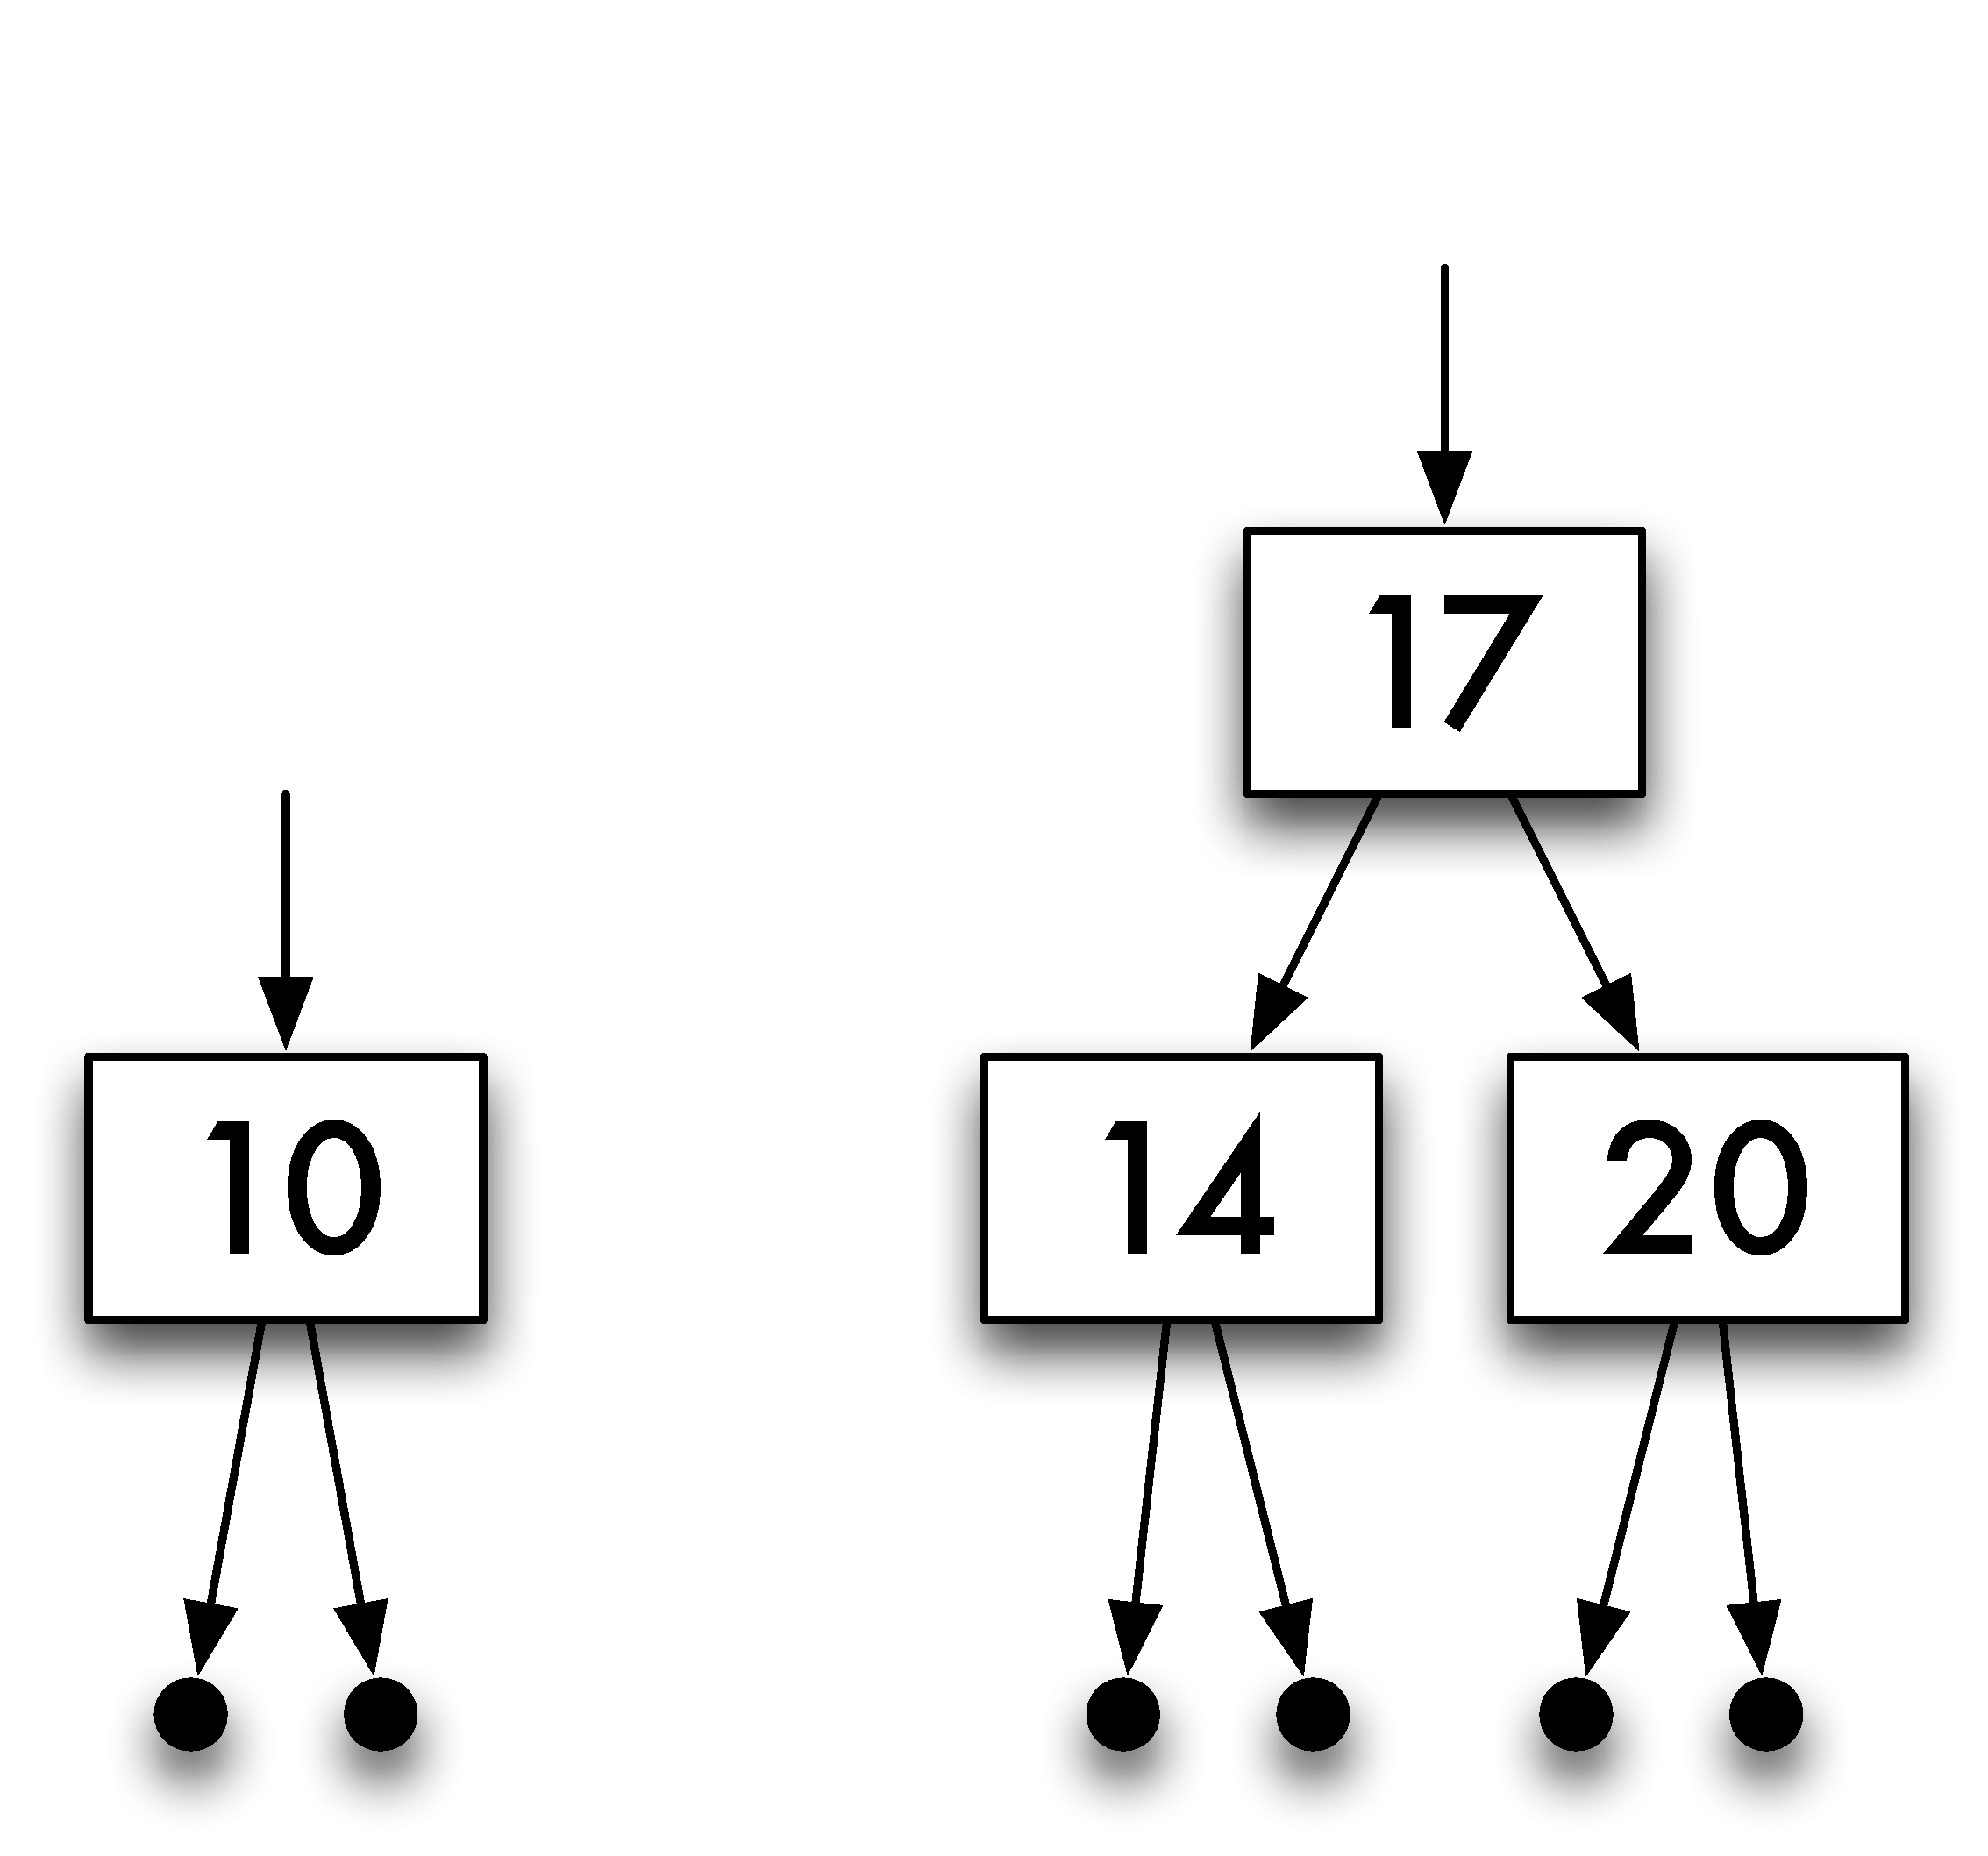
\includegraphics[width=3in]{Pictures/NewTwoTrees.pdf}
\end{center}
\caption{Two trees.}
\label{treeFig2}
\end{figure}
As a Haskell type we
say
\begin{alltt}
data NTree = NilT |\minx{NTree}
             Node Integer NTree NTree
\end{alltt}
Finally, we have already used the type of lists: a list is either empty (
\texttt{[]}) or is built from a head and a tail -- another list -- using the list
constructor `\texttt{:}'. Lists will provide a good guide to using recursive
(and polymorphic) definitions. In particular they suggest how `general'
polymorphic higher-order functions over other algebraic types are defined, and
how programs are verified.  We now look at some examples in more detail.

\subsection*{Expressions}
\index{expression type|see{\texttt{Expr}}}\index{calculator|(}

The type \texttt{Expr} gives a model of the simple numerical expressions discussed
above. These might be used in implementing a simple numerical calculator,
for instance. 
\begin{alltt}\minx{Expr}
data Expr = Lit Integer |
            Add Expr Expr |
            Sub Expr Expr
\end{alltt}
Some examples are

\begin{mytable}
\mi 2 & \mi Lit 2\\
\mi 2+3 & \mi Add (Lit 2) (Lit 3)\\
\mi (3-1)+3 & \mi Add (Sub (Lit 3) (Lit 1)) (Lit 3)  
\end{mytable}

\medskip
\noindent
where the informal expressions are listed in the left-hand column, and their
\texttt{Expr} forms in the right. Given an expression, we might want to
\begin{titemize}
\item evaluate it;
\item turn it into a string, which can then be printed;
\item estimate its size -- count the operators, say.
\end{titemize}
Each of these functions will be defined in the same way, using \textbf{primitive
recursion}.\index{primitive recursion}
As the type is itself recursive, it is not a surprise that the
functions which handle the type are also recursive. Also, the form of the
recursive definitions follows the recursion in the type definition. For
instance, to evaluate an operator expression we work out the values of the
arguments and combine the results using the operator.
\begin{alltt}
eval :: Expr -> Integer\minx{eval}

eval (Lit n)     = n
eval (Add e1 e2) = (eval e1) + (eval e2)
eval (Sub e1 e2) = (eval e1) - (eval e2)
\end{alltt}
Primitive recursive definitions have two parts:
\begin{titemize}
\item At the non-recursive, {\em base\/} cases -- \texttt{(Lit n)} here -- the
value is given outright. 
\index{primitive recursion!base case}
\item At the recursive cases, the values of the function at the
\index{primitive recursion!recursive case}
sub-expressions from which the expression is formed -- \texttt{eval e1} and 
\texttt{eval e2} here -- can be used in
calculating the result. 
\end{titemize}
The \texttt{show} function has a similar form
\begin{alltt}
show :: Expr -> String\index{show@\texttt{show}!\texttt{Expr}}

show (Lit n) = show n
show (Add e1 e2) 
  = "(" ++ show e1 ++ "+" ++ show e2 ++ ")"
show (Sub e1 e2) 
  = "(" ++ show e1 ++ "-" ++ show e2 ++ ")"
\end{alltt}
as does the function to calculate the number of operators in an expression;
we leave this as an exercise. Other exercises at the end of the section look
at a different representation of expressions for which a separate type is used
to represent the different possible operators. Next, we look at another
recursive algebraic type, but after that we return to \texttt{Expr} and give an
example of a non-primitive-recursive definition of a function to rearrange
expressions in a particular way.
\index{calculator|)}

\subsection*{Trees of integers}
\index{tree!numeric}

Trees of integers like that in Figure \ref{treeFig} can be modelled by the type
\begin{alltt}
data NTree = NilT |\minx{NTree}
             Node Integer NTree NTree
\end{alltt}
The null tree is given by \texttt{NilT}, and the trees in Figure \ref{treeFig2}
by
\begin{alltt}
Node 10 NilT NilT
Node 17 (Node 14 NilT NilT) (Node 20 NilT NilT)
\end{alltt}
Definitions of many functions are primitive recursive. For instance,
\index{primitive recursion}
\begin{alltt}
sumTree,depth :: NTree -> Integer\minx{sumTree}\minx{depth}

sumTree NilT           = 0
sumTree (Node n t1 t2) = n + sumTree t1 + sumTree t2

depth NilT             = 0
depth (Node n t1 t2)   = 1 + max (depth t1) (depth t2)
\end{alltt}
with, for example,
\begin{alltt}
sumTree (Node 3 (Node 4 NilT NilT) NilT) = 7
depth   (Node 3 (Node 4 NilT NilT) NilT) = 2
\end{alltt}
As another example, take the problem of finding out how many times a number,
\texttt{p} say, occurs in a tree. The primitive recursion suggests two cases,
depending upon the tree.
\begin{titemize} 
\item For a null tree, \texttt{NilT}, the answer must be zero.
\item For a non-null tree, \texttt{(Node n t1 t2)}, we can find out how many
times \texttt{p} occurs in the sub-trees \texttt{t1} and \texttt{t2} by two recursive
calls; we have to make a case split depending on whether \texttt{p} occurs at the
particular node, that is depending on whether or not \texttt{p==n}. 
\end{titemize}
The final definition is 
\begin{alltt}\minx{occurs}
occurs :: NTree -> Integer -> Integer

occurs NilT p = 0
occurs (Node n t1 t2) p
  | n==p        = 1 + occurs t1 p + occurs t2 p
  | otherwise   =     occurs t1 p + occurs t2 p
\end{alltt}

The exercises at the end of the section give a number of other
examples of functions defined over trees using primitive
recursion. We next look at a particular example where a
different form of recursion is used. 


\subsection*{Rearranging expressions}
%\index{expression type!rearranging}

The next example shows a definition which uses a more general recursion than
we have seen so far. After showing why the generality is necessary, we argue
that the function we have defined is total: it will give a result on all
well-defined expressions.

The operation of addition over the integers
is associative\index{associativity}, so that the way in which an
expression is bracketed is irrelevant to its value. We can, therefore, decide
to bracket expressions involving `\texttt{+}' in any way we choose. The aim here
is to write a program to turn expressions into right bracketed form, as shown in Figure \ref{associate} and
in the following table:
\begin{alltt}
(2+3)+4                 2+(3+4)
((2+3)+4)+5             2+(3+(4+5))
((2-((6+7)+8))+4)+5    (2-(6+(7+8)))+(4+5)
\end{alltt}
What is the program to do? The main aim is to spot occurrences of
\begin{alltt}\minx{Expr}
Add (Add e1 e2) e3 \hfill (AddL)
\end{alltt}
and to transform them to
\begin{alltt}
Add e1 (Add e2 e3)\hfill (AddR)
\end{alltt}
so a first attempt at the program might say
\begin{alltt}
try (Add (Add e1 e2) e3) 
  = Add (try e1) (Add (try e2) (try e3))
try ...
\end{alltt}
which is primitive recursive: on the right-hand side of their definition the
function \texttt{try} is only used on sub-expressions of the argument. This
function will have the effect of transforming \texttt{(AddL)} to \texttt{(AddR)}, but
unfortunately 
\texttt{(AddExL)} will be sent to \texttt{(AddExR)}:
\begin{alltt}
((2+3)+4)+5 \hfill (AddExL) 
(2+3)+(4+5)\hfill (AddExR)  
\end{alltt}

\begin{figure}[t]
\begin{center}
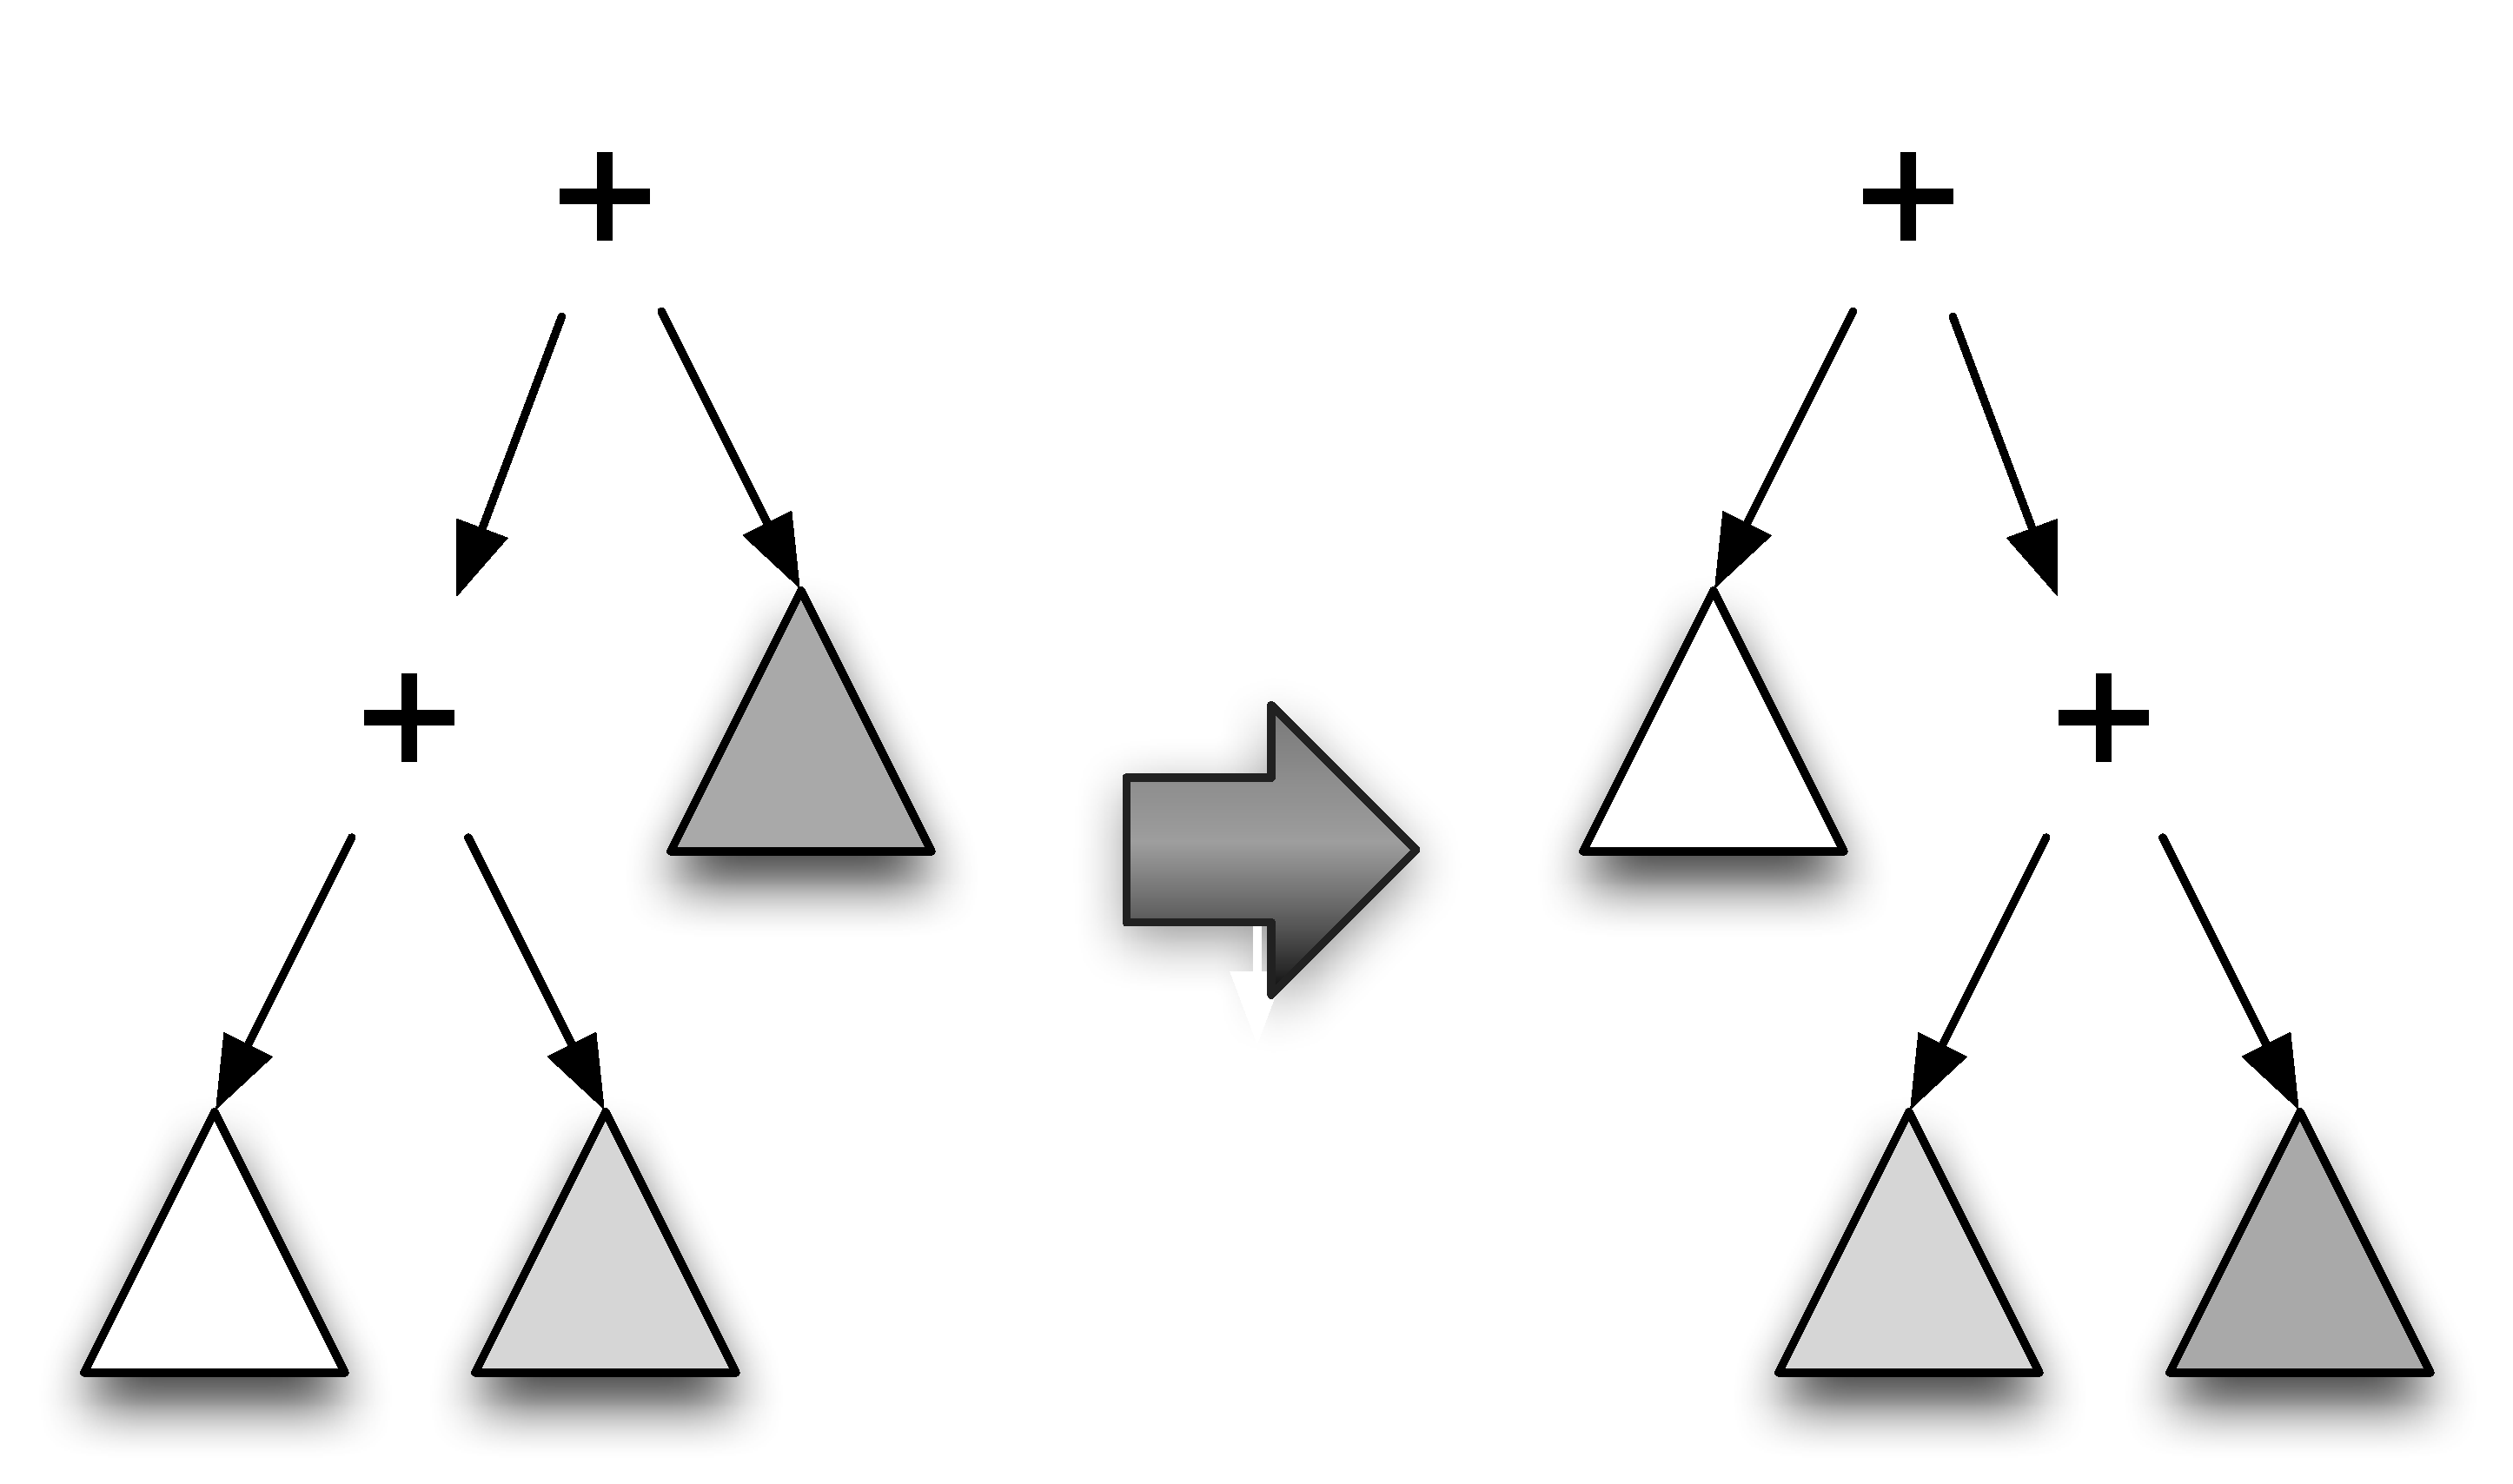
\includegraphics[width=3in]{Pictures/Associate.pdf}
\end{center}
\caption{Rearranging additions}
\label{associate}
\end{figure}

\noindent
The problem is that
in transforming \texttt{(AddL)} to \texttt{(AddR)} we may produce another pattern we are
looking for at the top level: this is precisely what happens when \texttt{(AddExL)}
is transformed to \texttt{(AddExR)}. We therefore have to call the function {\em again\/} on the
result of the rearrangement
\begin{alltt}
assoc :: Expr -> Expr\minx{assoc}

assoc (Add (Add e1 e2) e3)
  = assoc (Add e1 (Add e2 e3)) \hfill (Add.1)
\end{alltt}
The other cases in the definition make sure that the {\em parts\/} of an
expression are rearranged as they should be.
\begin{alltt}
assoc (Add e1 e2) 
  = Add (assoc e1) (assoc e2) \hfill (Add.2)
assoc (Sub e1 e2) 
  = Sub (assoc e1) (assoc e2)
assoc (Lit n) 
  = Lit n
\end{alltt}
The equation \texttt{(Add.2)} will only be applied to the cases where \texttt{(Add.1)} does
not apply -- this is when \texttt{e1} is either a \texttt{Sub} or a \texttt{Lit}
expression. This is always the case in pattern matching\index{pattern matching}; the {\em first\/}
applicable equation is used.

When we use primitive recursion we can be sure that the recursion will {\bf
terminate}\index{termination}
to give an answer: the  recursive calls are only made on smaller
expressions and so, after a finite number of calls to the function, a base
case will be reached. 

The \texttt{assoc} function is more complicated, and we
need a more subtle argument to see that the function will always give a
result. The equation \texttt{(Add.1)} is the tricky one, but intuitively, we can see
that some progress has been made -- some of the `weight' of the tree has moved
from left to right. In particular, one addition symbol has swapped sides.
None of the other equations moves a plus in the other direction, so
that after applying \texttt{(Add.1)} a finite number of times, there will be no more
exposed addition symbols at the top level of the left-hand side. This means
that the recursion cannot go on indefinitely, and so the function always
leads to a result.

In Section \ref{proofAlgTypes} we'll look at specifying QuickCheck properties for functions over algebraic types, including \texttt{assoc}, as well as showing how some of these can be proved by induction.

\subsection*{Syntax: infix constructors}
\index{constructor!infix}

We have seen that functions can be written in infix form; this also applies to
constructors. We can, for example, redefine the function \texttt{assoc} thus:
\begin{alltt}
assoc ((e1 `Add` e2) `Add` e3)
  = assoc (e1 `Add` (e2 `Add` e3))
 ...
\end{alltt}
using the infix form of the constructor, given by surrounding it with
back-quotes. 

When an expression like this is \texttt{show}n, it appears in prefix
form, so that the expression \texttt{(Lit 3) `Add` (Lit 4)} appears as
\begin{alltt}
Add (Lit 3) (Lit 4)
\end{alltt}
In a \texttt{data}
definition we can define Haskell operators which are themselves constructors. 
These constructors have the same syntax as
operator symbols, except that their first character must be a `\texttt{:}', which
is reminiscent of `\texttt{:}', itself an infix constructor. For our type of
integer expressions, we might define
\begin{alltt}
data Expr = Lit Integer |
            Expr :+: Expr |
            Expr :-: Expr
\end{alltt}
When an expression involving operator constructors is printed, the
constructors appear in the infix position, unlike the quoted constructors
above.

It is left as an exercise to complete the redefinition of functions over 
\texttt{Expr} under this redefinition of the \texttt{Expr} type.

\subsection*{Mutual recursion}
\index{recursion!mutual}
\index{recursive type!mutually recursive}

In describing one type, it is often useful to use others; these in turn may
refer back to the original type: this gives a pair of \textbf{mutually
recursive} types. A description of a person might include biographical
details,
which in turn might refer to other people. For instance: 
\begin{alltt}
data Person = Adult Name Address Bio |
              Child Name
data Bio    = Parent String [Person] |
              NonParent String
\end{alltt}
In the case of a
parent, the biography contains some text, as well as a list of their children,
as elements of the type \texttt{Person}.

Suppose that we want to define a function which shows information about a person as
a string. Showing this information will require us to show some biographical
information, which itself contains further information about people. We thus have two
mutually recursive functions:
\begin{alltt}
showPerson (Adult nm ad bio) 
  = show nm ++ show ad ++ showBio bio
  ...
showBio (Parent st perList)
  = st ++ concat (map showPerson perList)
  ...
\end{alltt}
\index{calculator|(}
\begin{exercises}

\item
Give calculations of 
\begin{alltt}
eval (Lit 67)
eval (Add (Sub (Lit 3) (Lit 1)) (Lit 3))
show (Add (Lit 67) (Lit (-34)))
\end{alltt}

\item
Define the function
\begin{alltt}
size :: Expr -> Integer
\end{alltt}
which counts the number of operators in an expression.

\item
Add the operations of multiplication and integer division to the type 
\texttt{Expr}, and redefine the functions \texttt{eval}, \texttt{show} and \texttt{size}
to include these new cases. What does your definition of \texttt{eval} do when
asked to perform a division by zero?

\item
Instead of adding extra constructors to the \texttt{Expr} type, as in the
previous question, it is possible to factor the definition thus:

\label{modExpr}\begin{alltt}
data Expr = Lit Integer |\minx{Expr}
            Op Ops Expr Expr

data Ops  = Add | Sub | Mul | Div \minx{Ops}
\end{alltt}
Show how the functions \texttt{eval}, \texttt{show} and \texttt{size} are defined
for this type, and discuss the changes you have to make to your definitions if
you add the extra operation \texttt{Mod} for remainder on integer division.

\item
Give line-by-line calculations of 
\begin{alltt}
sumTree (Node 3 (Node 4 NilT NilT) NilT)
depth   (Node 3 (Node 4 NilT NilT) NilT)
\end{alltt}

\item
Complete the redefinition of functions over \texttt{Expr} after it has been
defined using the infix constructors \texttt{:+:} and \texttt{:-:}.

\item
Define functions to return the left- and right-hand sub-trees
of an \texttt{NTree}.

\item
Define a function to decide whether a number is an element of an \texttt{NTree}.

\item
Define functions to find the maximum and minimum values held in an 
\texttt{NTree}.

\item
A tree is reflected by swapping left and right sub-trees, recursively. Define\break
a function to reflect an \texttt{NTree}. What is the result of
reflecting twice,\break \texttt{reflect .\ reflect}?

\item
Define functions
\begin{alltt}
collapse, sort :: NTree -> [Integer]
\end{alltt}
which turn a tree into a list. The function \texttt{collapse} should enumerate the
left sub-tree, then the value at the node and finally the right sub-tree;
\texttt{sort} should sort the elements in ascending order. For instance, 
\begin{alltt}
collapse (Node 3 (Node 4 NilT NilT) NilT) = [4,3]
sort     (Node 3 (Node 4 NilT NilT) NilT) = [3,4]
\end{alltt}

\item
Complete the definitions of \texttt{showPerson} and \texttt{showBio} which were
left incomplete in the text.

\item
It is possible to extend the type \texttt{Expr} so that it contains
{\em conditional \/}
expressions, \texttt{If b e1 e2},
where \texttt{e1} and \texttt{e2} are expressions, and
\texttt{b} is a Boolean expression, a member of the type \texttt{BExp},
\begin{alltt}
data Expr = Lit Integer |\minx{Expr}
            Op Ops Expr Expr |
            If BExp Expr Expr
\end{alltt}
The expression
\begin{alltt}
If b e1 e2
\end{alltt}
has the value of \texttt{e1} if \texttt{b} has the
value \texttt{True} and otherwise it has the value of \texttt{e2}.
\begin{alltt}
data BExp = BoolLit Bool |\minx{BExp}
            And BExp BExp |
            Not BExp |
            Equal Expr Expr |
            Greater Expr Expr
\end{alltt}
The five clauses here give
\begin{titemize}
\item Boolean literals, \texttt{BoolLit True} and \texttt{BoolLit False}.
\item The conjunction of two expressions; it is \texttt{True} if both sub-expressions have
the value \texttt{True}.
\item The negation of an expression. \texttt{Not be} has value \texttt{True} if
\texttt{be} has the value \texttt{False}.
\item \texttt{Equal e1 e2} is \texttt{True} when the two numerical expressions have
equal values.
\item \texttt{Greater e1 e2} is \texttt{True} when the numerical expression 
\texttt{e1} has a larger value then \texttt{e2}.
\end{titemize}
Define the functions 
\begin{alltt}
eval  :: Expr -> Integer \minx{eval}
bEval :: BExp -> Bool\minx{bEval}
\end{alltt}
by mutual recursion, and
extend the function \texttt{show} to show the redefined type of expressions.
\index{recursive type|)}
\index{calculator|)}
\end{exercises}
\section{Polymorphic algebraic types}
\label{polyAlg}
\index{algebraic type!polymorphic|(}


Algebraic type definitions can contain the type variables \texttt{a}, \texttt{b}
and so on, defining polymorphic types. The definitions are as before, with the
type variables used in the definition appearing after the type name on the 
left-hand side of the definition. A simple example is
\begin{alltt}
data Pairs a = Pr a a\minx{Pairs}
\end{alltt}
and example elements of the type are
\begin{alltt}
Pr 2 3    :: Pairs Integer
Pr [] [3] :: Pairs [Int]
Pr [] []  :: Pairs [a]
\end{alltt}
A function to test the equality of the two halves of a pair is given by
\begin{alltt}\minx{equalPair}
equalPair :: Eq a => Pairs a -> Bool
equalPair (Pr x y) = (x==y)
\end{alltt}
The remainder of this section explores a sequence of further examples.

\subsection*{Lists}
\index{lists!algebraic type of}


The built-in type of lists can be given by a definition like
\begin{alltt}\minx{List}\minx{:::}
infixr 5 :::

data List a = NilL | a ::: (List a)
              deriving (Eq,Ord,Show,Read)
\end{alltt}
where the syntax \texttt{[a]}, \texttt{[]} and `\texttt{:}' is used for \texttt{List a},
\texttt{NilList} and \texttt{:::}. Note that we have given a \textbf{fixity declaration} for \texttt{:::} to give it the same fixity and associativity as \texttt{:}, we can therefore write expressions like this:\index{fixity!declaration}
\begin{alltt}
\textsl{*Chapter14>} 2+3 ::: 4+5 ::: NilL
\textsl{5 ::: (9 ::: NilL)}
\end{alltt}
much as lists are written with \texttt{:}.

Lists form a useful paradigm
for recursive polymorphic types. In particular, we can see the possibility of
defining useful families of functions over such types, and the way in which
program verification can proceed by induction over the structure of a type.

\subsection*{Binary trees}
\index{tree!binary}\index{binary tree|see{tree}}

The trees of Section \ref{recTypes} carry numbers at each node; there is
nothing special about numbers, and we can equally well say that
they have elements of an arbitrary type at the nodes:
\begin{alltt}\minx{Nil}\minx{Node}
data Tree a = Nil | Node a (Tree a) (Tree a)\minx{Tree}
              deriving (Eq,Ord,Show,Read)
\end{alltt}
The definitions of \texttt{depth} and \texttt{occurs} carry over unchanged:
\begin{alltt}
depth :: Tree a -> Integer\minx{depth}
depth Nil            = 0
depth (Node n t1 t2) = 1 + max (depth t1) (depth t2)
\end{alltt}
as do many of the functions defined in the exercises at the end of Section
\ref{recTypes}.  
One of these is the function collapsing a tree into a list. This is done
by visiting the elements of the tree `inorder', that is visiting first the left
sub-tree, then the node itself, then the right sub-tree, thus:
\begin{alltt}
collapse :: Tree a -> [a]\minx{collapse}
collapse Nil = []
collapse (Node x t1 t2)
  = collapse t1 ++ [x] ++ collapse t2
\end{alltt}
For example,
\begin{alltt}
collapse (Node 12 
               (Node 34 Nil Nil) 
               (Node 3 (Node 17 Nil Nil) Nil))
  = [34,12,17,3]
\end{alltt}
Various higher-order functions are definable, also,
\begin{alltt}
mapTree :: (a -> b) -> Tree a -> Tree b\minx{mapTree}
mapTree f Nil = Nil
mapTree f (Node x t1 t2)
  = Node (f x) (mapTree f t1) (mapTree f t2)
\end{alltt}
We shall return to trees in Section \ref{srchTrees}, where
particular `search' trees form a case study.


\subsection*{The union type, \texttt{Either}}
\index{union type}\index{sum type}

Type definitions can take more than one parameter. We saw earlier the example
of the type whose elements were either a name or a number. In general we can
form a type whose elements come either from \texttt{a} or from \texttt{b}:
\begin{alltt}\minx{Left}\minx{Right}
data Either a b = Left a | Right b
                  deriving (Eq,Ord,Read,Show)\minx{Either}
\end{alltt}
Members of the `union' or `sum' type are \texttt{(Left x)}, with
\texttt{x::a}, and
\texttt{(Right y)} with \texttt{y::b}. The `name or number' type is given by 
\texttt{Either String Int} and
\begin{alltt}
Left "Duke of Prunes" :: Either String Int
Right 33312           :: Either String Int
\end{alltt}
We can tell whether an element is in the first half of the 
union by\minx{isLeft}
\begin{alltt} 
isLeft :: Either a b -> Bool
isLeft (Left _)  = True
isLeft (Right _) = False
\end{alltt}
To define a function from \texttt{Either a b} to \texttt{Int}, say, we have to deal
with two cases,
\begin{alltt}
fun :: Either a b -> Int
fun (Left x)  = ... x ...
fun (Right y) = ... y ...
\end{alltt}
In the first case, the right-hand side takes \texttt{x} to an \texttt{Int}, so is
given by
a function from \texttt{a} to \texttt{Int}; in the second case \texttt{y} is taken to
an \texttt{Int}, thus being given by a function from \texttt{b} to \texttt{Int}. 

Guided by this, we can give a higher-order
function which {\em joins together\/} two functions defined on \texttt{a} and 
\texttt{b} to a function on \texttt{Either a b}. The definition follows, and is
illustrated in Figure \ref{either}.
\begin{figure}[t]
\begin{center}
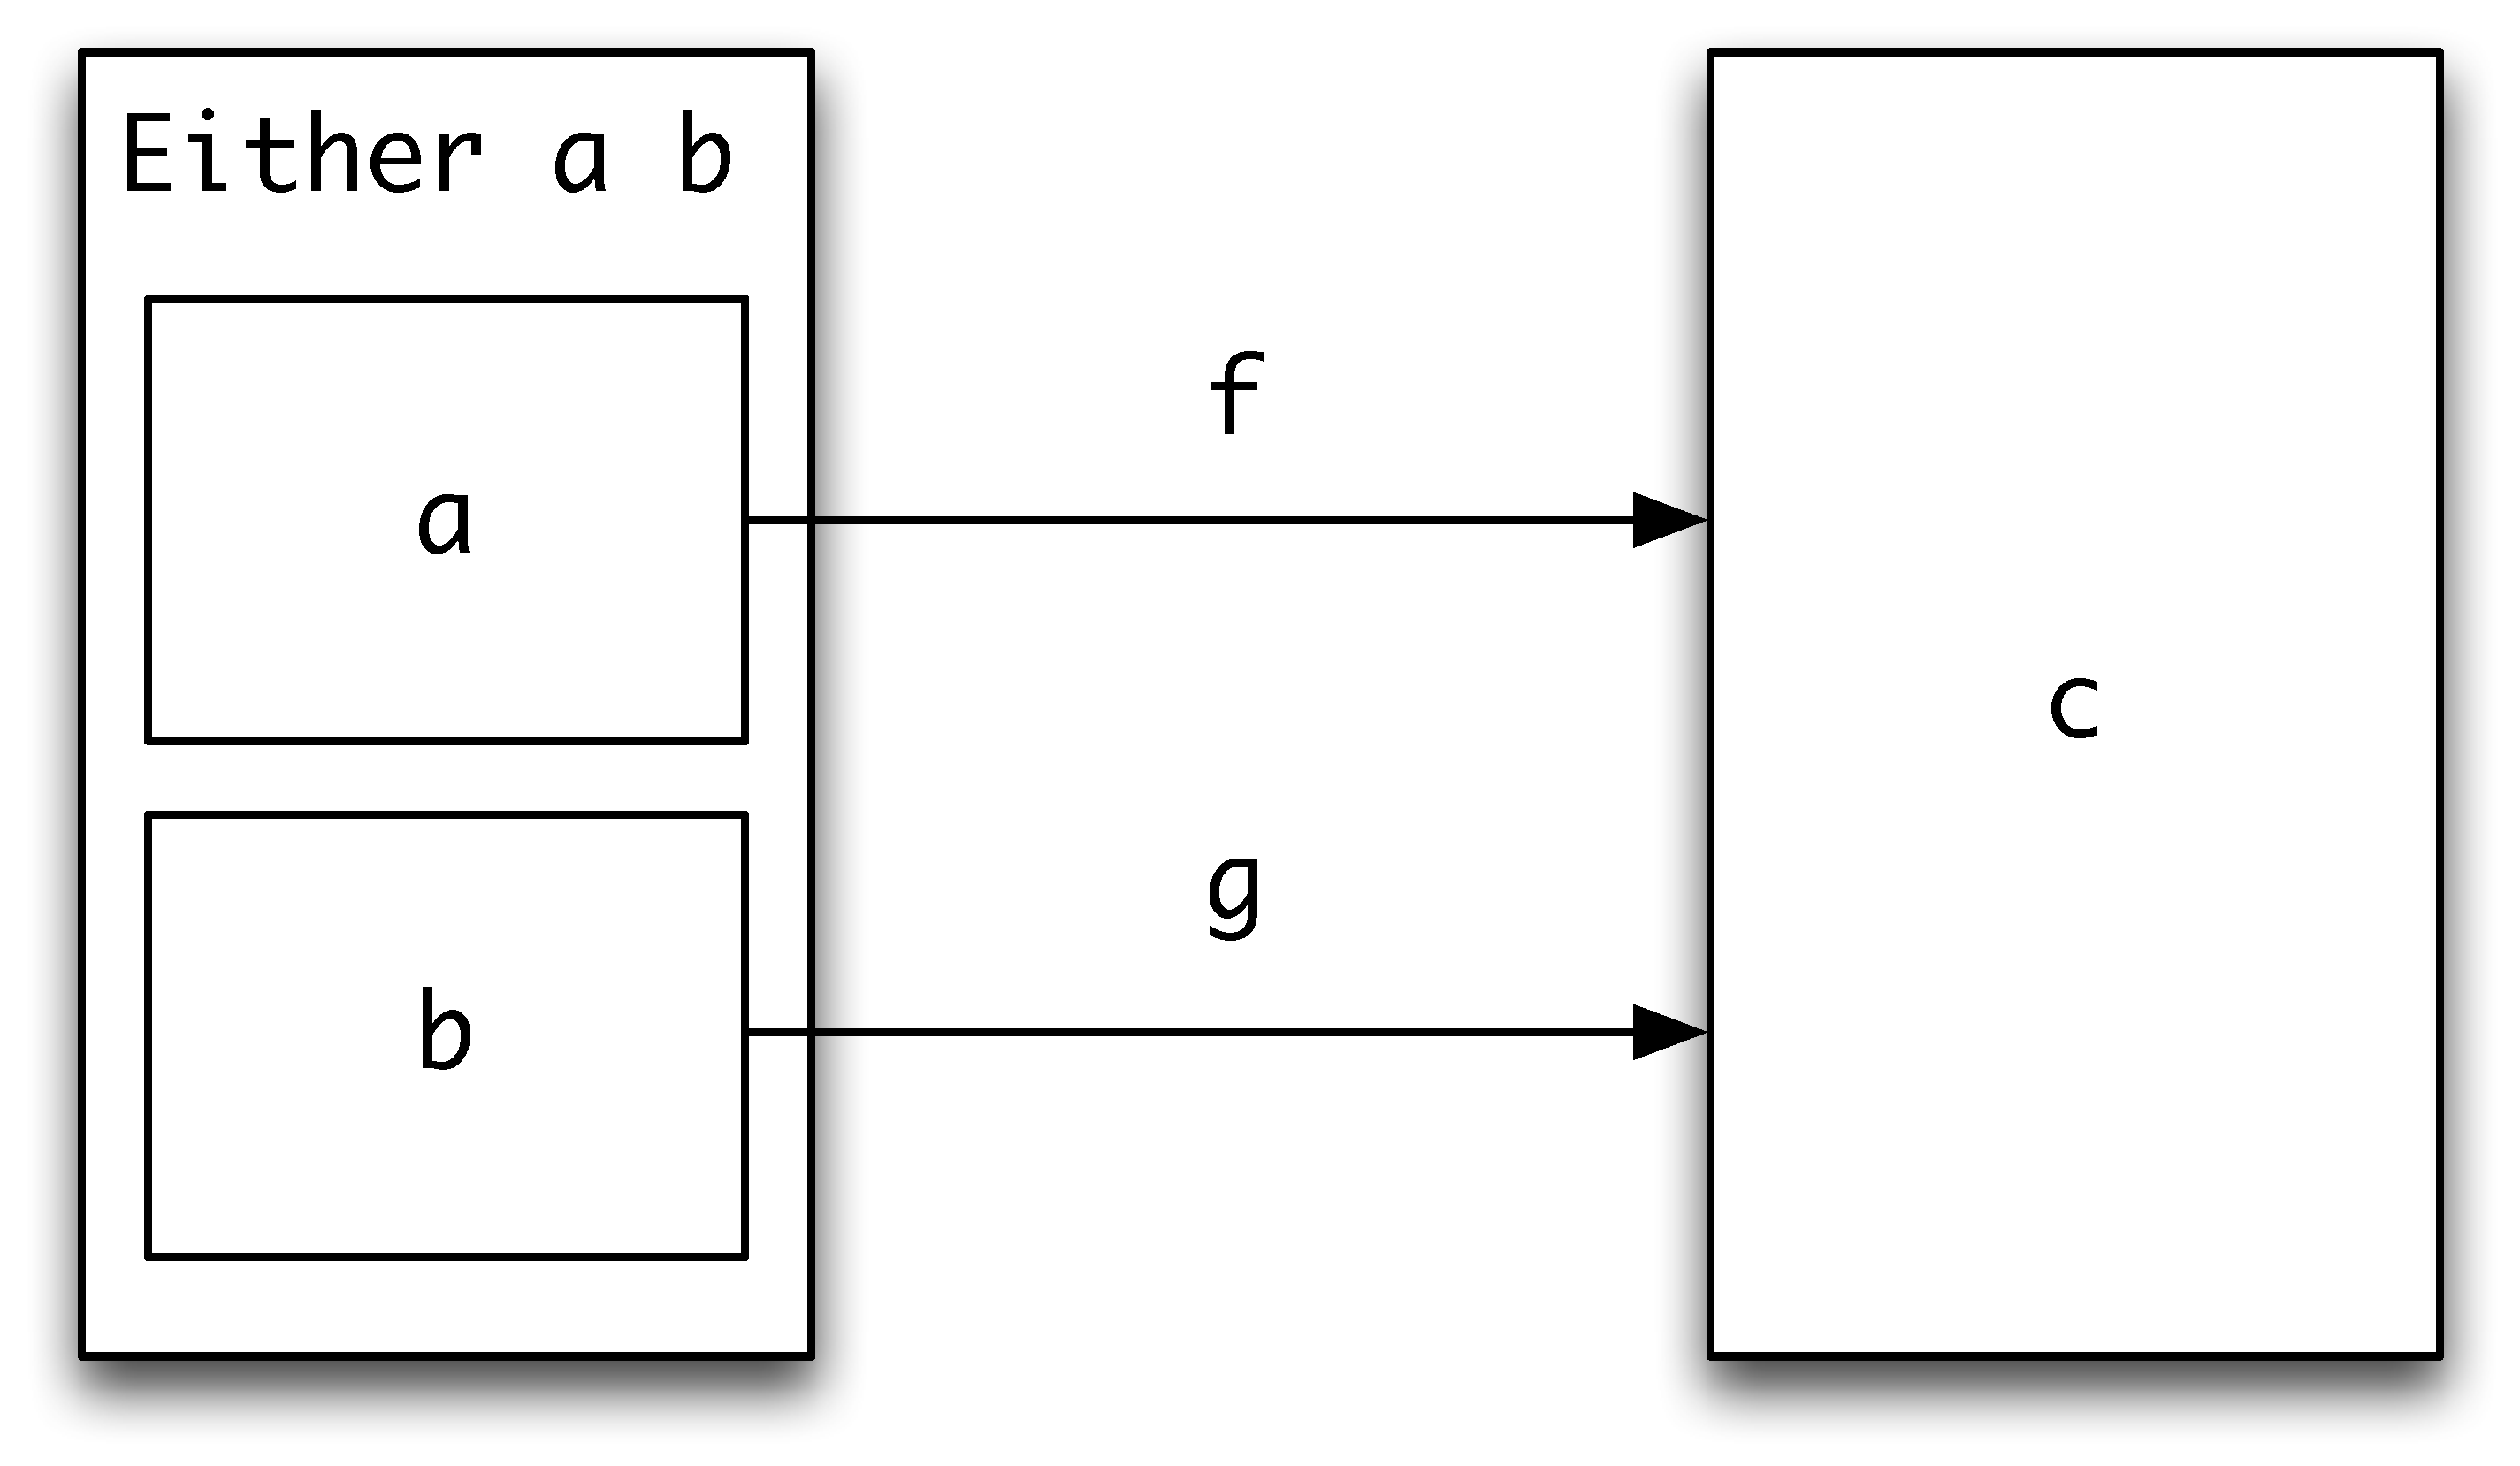
\includegraphics[width=3in]{Pictures/either1}
\end{center}
\label{either}
\caption{Joining together functions.}
\end{figure} 
\begin{alltt}\minx{either}
either :: (a -> c) -> (b -> c) -> Either a b -> c

either f g (Left x)  = f x
either f g (Right y) = g y
\end{alltt}
If we have a function \texttt{f::a -> c} and we wish to apply it to an element
of \mbox{\texttt{Either a b}}, there is a problem: what do we do if the element is
in the right-hand side of the \texttt{Either} type? 
A simple answer is to raise an \texttt{error}
\begin{alltt}\minx{applyLeft}
applyLeft :: (a -> c) -> Either a b -> c
applyLeft f (Left x)  = f x
applyLeft f (Right _) = error "applyLeft applied to Right"
\end{alltt}
but in the next section we shall explore other ways of handling errors in more
detail.

\index{algebraic type!polymorphic|)}
\begin{exercises}

\item
Investigate which of the functions over trees discussed in the exercises of
Section \ref{recTypes} can be made polymorphic.

\item
Define a function \texttt{twist} which swaps the order of a union
\begin{alltt}
twist :: Either a b -> Either b a
\end{alltt}
What is the effect of \texttt{(twist .\ twist)}?

\item
How would you define \texttt{applyLeft} using the function
\texttt{either}?

\item
Show that any function of type \texttt{a -> b} can be transformed into
functions of type
\begin{alltt}
a -> Either b c
a -> Either c b
\end{alltt}

\item
How could you generalize \texttt{either} to \texttt{join} so that it has type
\begin{alltt}
join :: (a -> c) -> (b -> d) -> Either a b -> Either c d
\end{alltt}
You might find the answer to the previous exercise useful here, if you want
to define \texttt{join} using \texttt{either}.
\end{exercises}

\medskip\noindent
The trees defined in the text are {\em binary}: each non-nil
tree has exactly two
sub-trees. We can instead define general
trees with an arbitrary list of sub-trees,
thus:
\begin{alltt}
data GTree a = Leaf a | Gnode [GTree a]\minx{GTree}
\end{alltt}
The exercises which follow concern these trees.

\begin{exercises}
\item
Define functions 
\begin{titemize} 
\item to count the number of leaves in a \texttt{GTree}; 
\item to find
the depth of a \texttt{GTree}; 
\item to sum a numeric \texttt{GTree Int}; 
\item to find whether
an element appears in a \texttt{GTree}; 
\item to map a function over the elements at
the leaves of a \texttt{GTree}; and 
\item to flatten a \texttt{GTree} to a list.
\end{titemize}
In each case give the type of the function that you have defined.
\item
How is the completely empty tree represented as a \texttt{GTree}?

\end{exercises}
\section{Modelling program errors}
\label{progErrs}
\index{error handling|(}

\noindent
How should a program deal with a situation which ought not to occur? Examples
of such situations include
\begin{titemize}
\item attempts to divide by zero, to take the square root of a negative
number, and other arithmetical transgressions;
\item attempts to take the head of an empty list -- this is a special case
of a definition over an algebraic type from which one case (here the empty
list) is absent.
\end{titemize}
This section examines the problem, giving three approaches of increasing
sophistication. The simplest method is to stop computation  and to report the
source of  the problem. This is indeed what the Haskell system does in the
cases listed above, and we can do this in functions we define ourselves using
the \texttt{error} function,
\begin{alltt}
error :: String -> a\minx{error}
\end{alltt}
An attempt to evaluate the expression 
\texttt{error "Circle with negative radius"}
in GHCi results in the message 
\begin{alltt}
*** Exception: Circle with negative radius
\end{alltt}
being printed and computation stopping.

The problem with this approach is that all the useful information in the
computation is lost; instead of this, the error can be dealt with in some way
{\em without\/} stopping computation completely. Two approaches suggest
themselves, and we look at them in turn now.

\subsection*{Dummy values}
\index{dummy values at errors}

The function \texttt{tail} is supposed to give the tail of a list, and it gives an
error message on an empty list:
\begin{alltt}
tail :: [a] -> [a]\minx{tail}
tail (_:xs) = xs
tail []     = error "Prelude.tail: empty list"
\end{alltt}
We could redefine it to say
\begin{alltt}
tl :: [a] -> [a]\minx{tl}
tl (_:xs) = xs
tl []     = []
\end{alltt}
Now, an attempt to take the tail of {\em any\/} list will succeed. In a
similar way we could say
\begin{alltt}
divide :: Integer -> Integer -> Integer
divide n m 
  | (m /= 0)    = n `div` m
  | otherwise   = 0
\end{alltt}
so that division by zero gives some answer. For \texttt{tl} and \texttt{divide}
there have been obvious choices about what the value in the `error' case
should be; for \texttt{head} there is not, and instead we can supply an extra
parameter to \texttt{head}, which is to be used in the case of the list being
empty.
\begin{alltt}\minx{hd}
hd :: a -> [a] -> a
hd y (x:_) = x
hd y []    = y
\end{alltt}
This approach is completely general; if a function \texttt{f} (of one
argument, say) usually raises an error when \texttt{cond} is \texttt{True}, we can
define a new function
\begin{alltt}
fErr y x 
  | cond        = y
  | otherwise   = f x
\end{alltt}
This approach works well in many cases; the only drawback is that we have no
way of telling when an error has occurred, since we may get the result 
\texttt{y} from either the error or the `normal' case.
Alternatively we can use an error type to trap and process errors; this
we look at now.

\subsection*{Error types}
\index{error handling!error type}
\minx{Maybe}

The previous approach works by returning a dummy value when an error has
occurred. Why not instead return an error {\em value\/} as a result? We
define the type
\begin{alltt}\minx{Nothing}\minx{Just}
data Maybe a = Nothing | Just a\minx{Maybe}
               deriving (Eq,Ord,Read,Show)
\end{alltt}
which is effectively the type \texttt{a} with an extra value \texttt{Nothing} added.
We can now define a division function \texttt{errDiv} thus
\begin{alltt}\minx{errDiv}
errDiv :: Integer -> Integer -> Maybe Integer
errDiv n m 
  | (m /= 0)    = Just (n `div` m)
  | otherwise   = Nothing 
\end{alltt}
and in the general case, where \texttt{f} gives an error when \texttt{cond} holds,
\begin{alltt}
fErr x 
  | cond        = Nothing
  | otherwise   = Just (f x)
\end{alltt}
The results of these functions are now not of the original output type, \texttt{a}
say, but
of type \texttt{Maybe a}. These \texttt{Maybe} types allow us to \textbf{raise} an error,
potentially. We can do two things with a potential error which has been 
raised
\begin{titemize}
\item we can {\em transmit\/} the error through a function, the effect
of \texttt{mapMaybe};\minx{mapMaybe}
\index{error handling!error transmission}
\item we can {\em trap\/} an error, the role of \texttt{maybe}.
\index{error handling!error trapping}\minx{maybe}
\end{titemize}
These two operations are illustrated in Figure \ref{errPic}, and we define them now.

The function \texttt{mapMaybe} transmits an error value through the application of
the function \texttt{g}. Suppose that \texttt{g} is a function of type \texttt{a -> b}, and that
we are to lift it to operate on the type \texttt{Maybe a}. In the case
of an argument
\texttt{Just x}, \texttt{g} can be
applied to the \texttt{x} to give a result, \texttt{g x}, of type \texttt{b}; this is put 
into \texttt{Maybe b}
by applying  the constructor function \texttt{Just}. On the other hand, if \texttt{Nothing} is the argument then 
\texttt{Nothing} is the result.
\begin{alltt}
mapMaybe :: (a -> b) -> Maybe a -> Maybe b\minx{mapMaybe}

mapMaybe g Nothing  = Nothing
mapMaybe g (Just x) = Just (g x)
\end{alltt}
In trapping an error, we aim to return a result of type \texttt{b}, from an
input of type \texttt{Maybe a}; we have two cases to deal with
\begin{titemize}
\item in the \texttt{Just} case, we apply a function from \texttt{a} to \texttt{b};
\item in the \texttt{Nothing} case, we have to give the value of type \texttt{b} which
is to be returned. (This is rather like the value we
supplied to \texttt{hd} earlier.)
\end{titemize}
The higher-order function which achieves this
is \texttt{maybe}, whose arguments \texttt{n} and \texttt{f} are used in the \texttt{Nothing}
and \texttt{Just} cases respectively. 
\begin{figure}[t]
\begin{center}
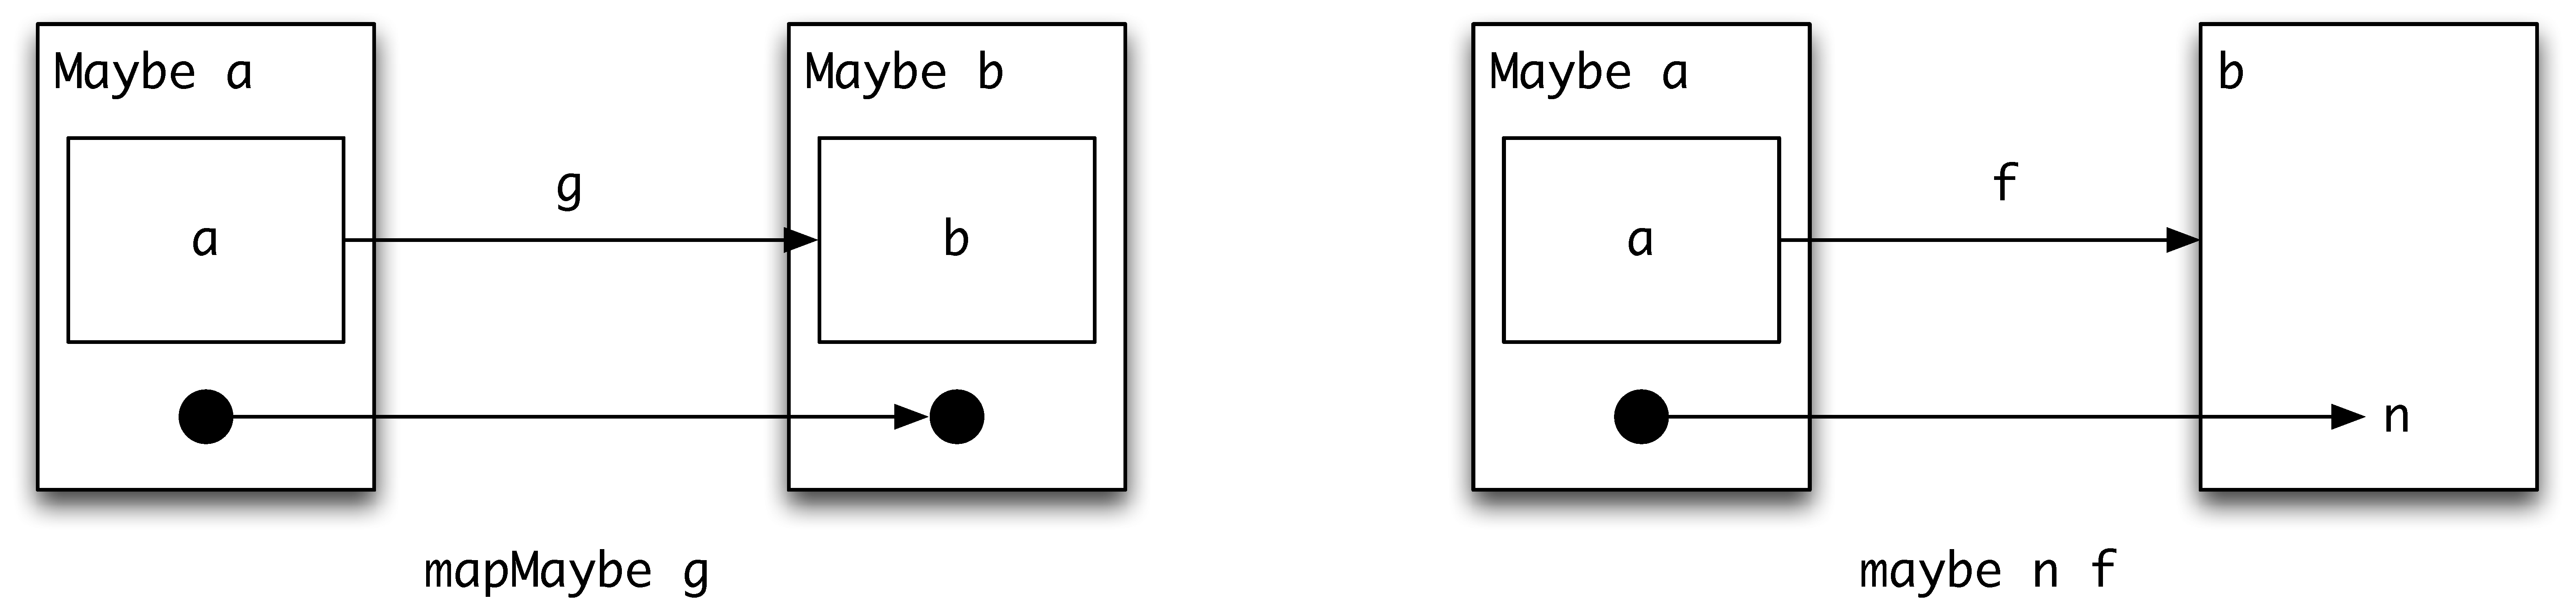
\includegraphics[width=5in]{Pictures/maybe1.pdf}
\end{center}
\label{errPic}
\caption{Error-handling functions.}
\end{figure}
\begin{alltt}
maybe :: b -> (a -> b) -> Maybe a -> b\minx{maybe}

maybe n f Nothing  = n
maybe n f (Just x) = f x
\end{alltt}
We can see the functions \texttt{mapMaybe} and \texttt{maybe} in action in the examples 
which follow. In the first, a division by zero leads to a \texttt{Nothing} which
passes through the lifting to be trapped -- \texttt{56} is therefore returned:
\begin{alltt}
maybe 56 (1+) (mapMaybe (*3) (errDiv 9 0)) 
= maybe 56 (1+) (mapMaybe (*3) Nothing)
= maybe 56 (1+) Nothing
= 56
\end{alltt}
In the second, a normal division returns a \texttt{Just 9}. This is multiplied by
three, and the \texttt{maybe} at the outer level adds one and removes the 
\texttt{Just}:
\begin{alltt}
maybe 56 (1+) (mapMaybe (*3) (errDiv 9 1))  
= maybe 56 (1+) (mapMaybe (*3) (Just 9)) 
= maybe 56 (1+) (Just 27)
= 1 + 27 
= 28
\end{alltt}
\index{design!error handling}
The advantage of the approach discussed here is that we can first define the
system without error handling, and afterwards add the error handling, using
the \texttt{mapMaybe} and \texttt{maybe} functions together with the modified functions
to \textbf{raise} the error. As we have seen numerous times already, separating
a problem into two parts has made the solution of each, and therefore the
whole, more accessible.

We revisit the \texttt{Maybe} type in Section \ref{monadFP} where we see that 
it is
an example of a more general programming structure, a monad. In
particular there we examine the relationship between the function
\texttt{mapMaybe} and the \texttt{map} function over lists.

\begin{exercises}

\item
Using the functions \texttt{mapMaybe} and \texttt{maybe}, or otherwise, define a function 
\begin{alltt}
process :: [Int] -> Int -> Int -> Int
\end{alltt}
so that \texttt{process xs n m} takes the \texttt{n}th and \texttt{m}th items of the list
of numbers \texttt{xs}, and returns their sum. Your function should return \texttt{0}
if either of the numbers is not one of the indices of the list:
for a list of length \texttt{p}, the indices are \texttt{0}, \ldots, 
\texttt{p-1} inclusive.

\item
Discuss the advantages and disadvantages of the three approaches to error
handling presented in this section.

\item
What are the values of type \texttt{Maybe (Maybe a)}?
Define a function
\begin{alltt}\minx{squashMaybe}
squashMaybe :: Maybe (Maybe a) -> Maybe a
\end{alltt}
which will `squash' \texttt{Just (Just x)} to \texttt{Just x} and all other values to
\texttt{Nothing}.

\item
In a similar way to \texttt{mapMaybe}, define the function
\begin{alltt}\minx{composeMaybe}
composeMaybe :: (a -> Maybe b) -> 
                (b -> Maybe c) -> 
                (a -> Maybe c)
\end{alltt}
which composes two error-raising functions. How could you use \texttt{mapMaybe}, the
function composition operator
and the \texttt{squash} function to define \texttt{composeMaybe}?

\item
The \texttt{Maybe} type could be generalized to allow messages to be carried in the
\texttt{Nothing} part, thus: 
\begin{alltt}
data Err a = OK a | Error String\minx{Err}
\end{alltt}
How do the definitions of \texttt{mapMaybe}, \texttt{maybe} and \texttt{composeMaybe} have to
be modified to accommodate this new definition?
\index{error handling|)}
\end{exercises}
\section{Design with algebraic data types}
\label{algDesign}
\index{design!and algebraic types|(}

Algebraic data types provide us with a powerful mechanism for modelling types
which occur both in problems themselves, and within the programs
designed to solve them. In this section we suggest a three-stage method for
finding the appropriate algebraic type definitions. We apply it in two
examples: finding the `edit distance' between two words, and a simulation problem.

An important moral of the discussion here is that we can start to design
data types 
{\em independently\/} of the program itself. For a system of any size
we should do this, as we will be more likely to succeed if we can think about
separate parts of the system separately. 

We shall have more to say about design of data types in the next two chapters.

\subsection*{Edit distance: problem statement}
\index{examples!edit distance|see{edit distance}}
\index{edit distance|(}

In discussing the stages of design, 
we follow the example of finding the \textbf{edit distance} between two
strings. This is the shortest sequence of simple editing operations which can
take us from one string to the other. 
 
The example is a version of a practical
problem: in keeping a display (of windows or simple text) up-to-date, the
speed with which updates can be done is crucial. It is therefore desirable to
be able to make the updates from as few elementary operations as possible;
this is what the edit distance program achieves in a different context.

We suppose that there are five basic editing operations on a string. We can
change one character into another, copy a character without modifying it,
delete or insert a character and delete (kill) to the end of the string. We
also assume that each operation has the same cost, except a copy which is
free. 

\begin{wrapfigure}[19]{l}{4cm}
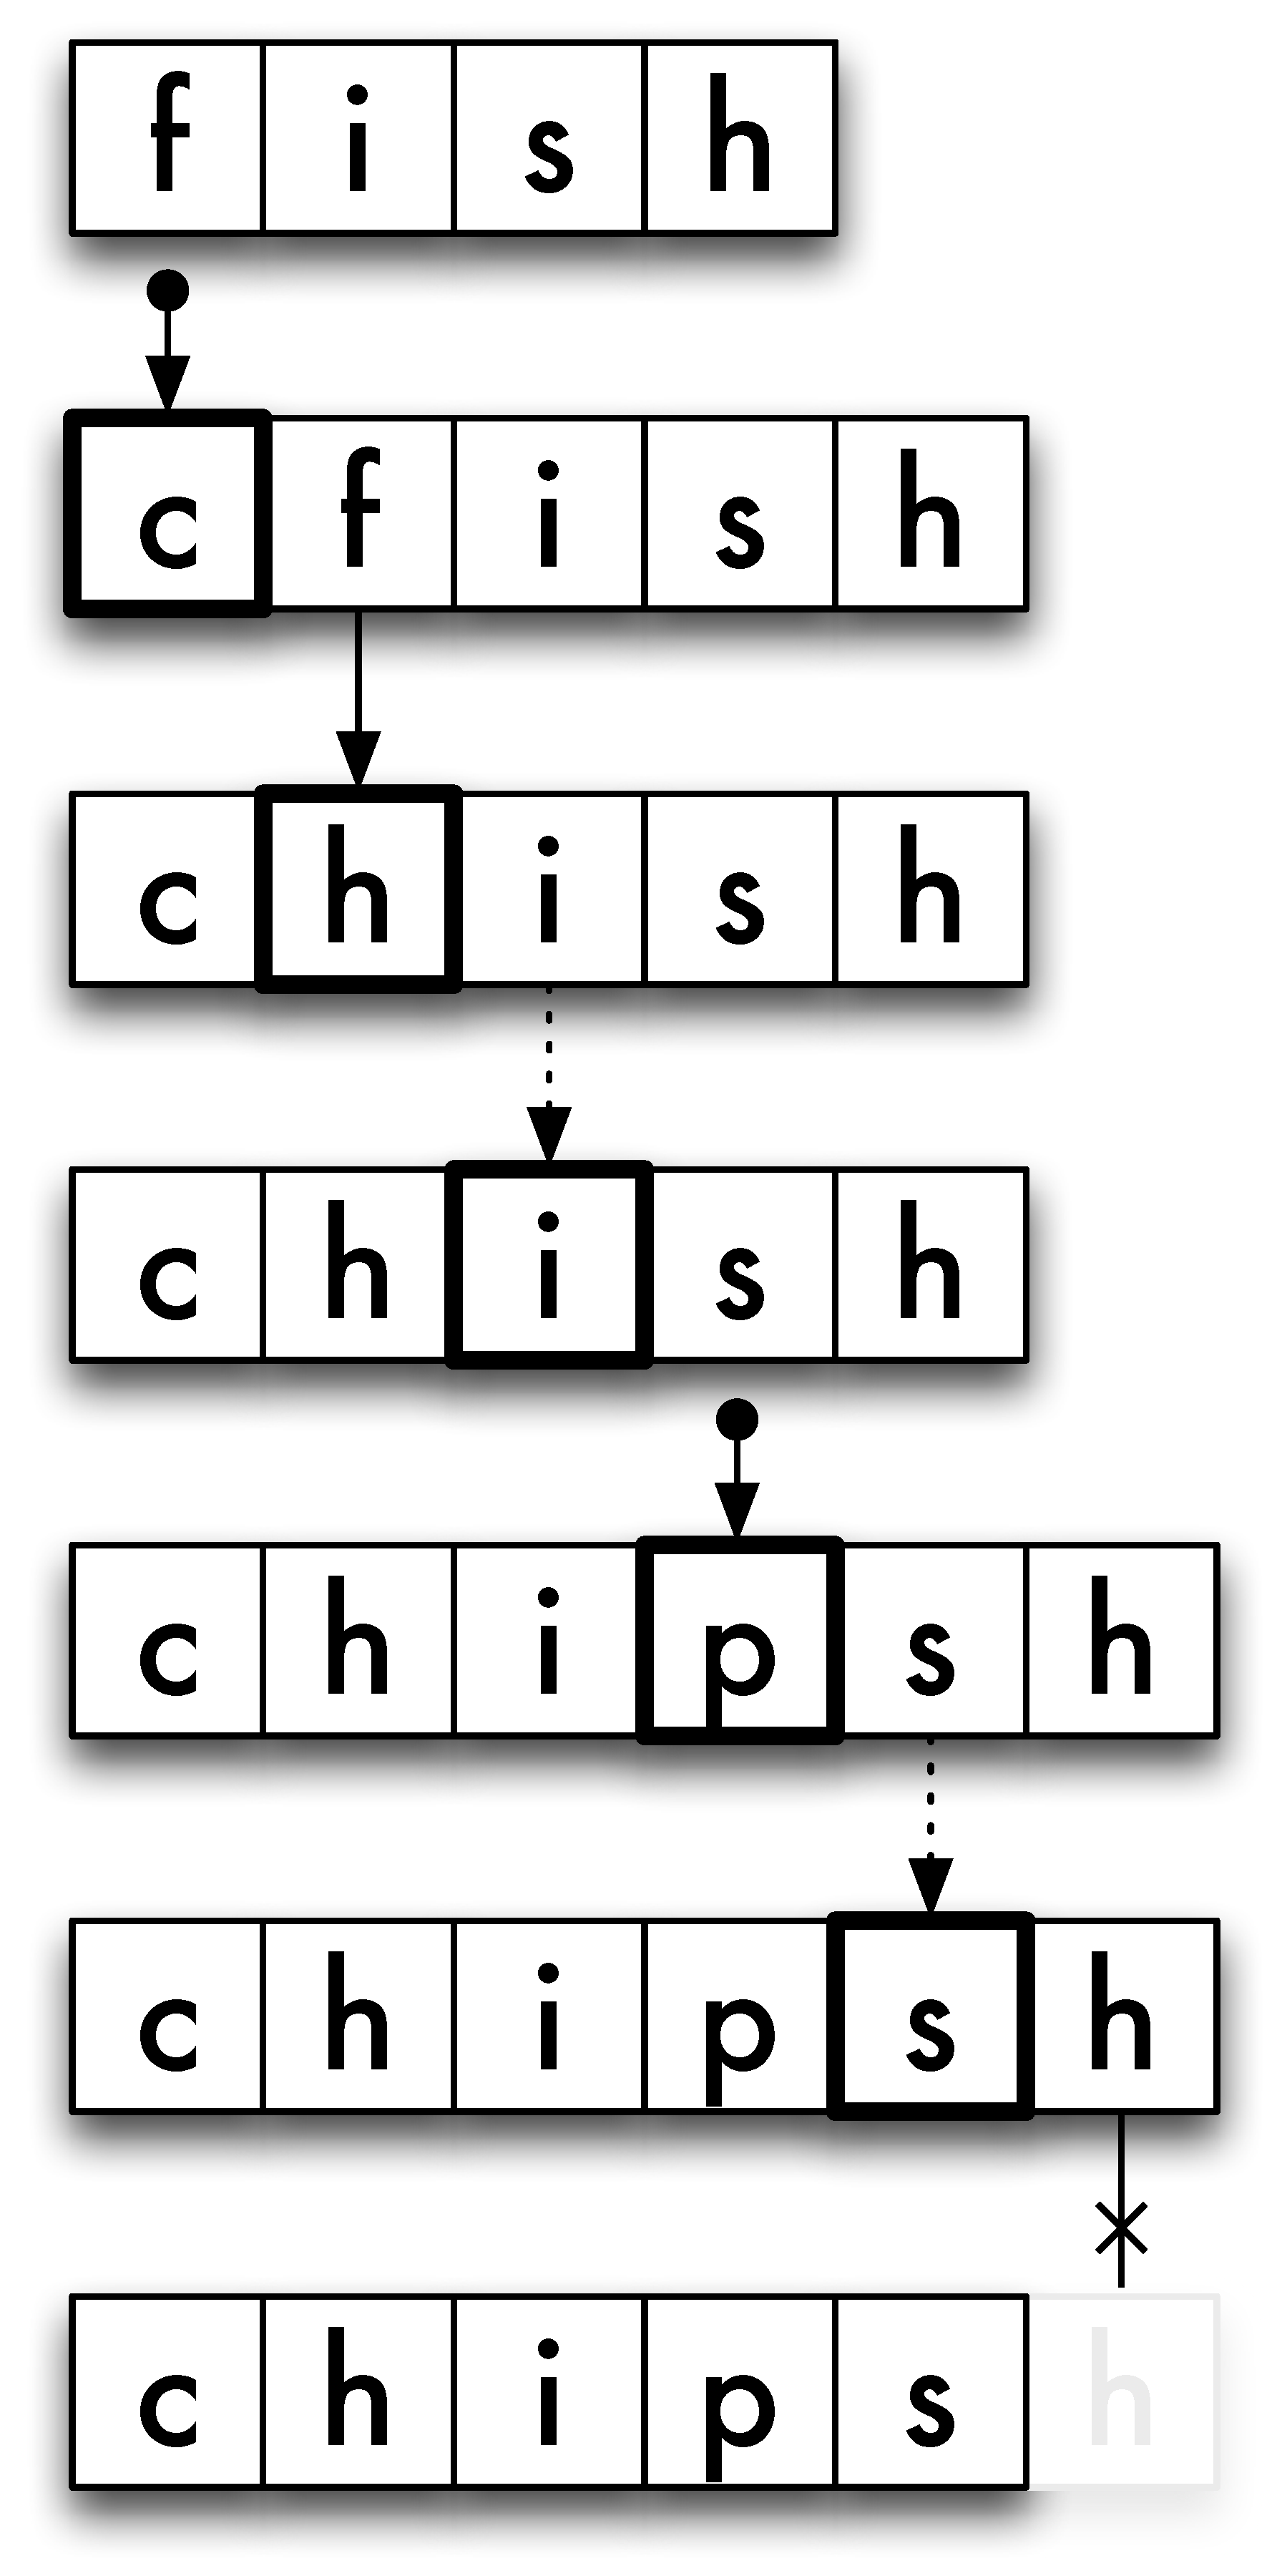
\includegraphics[width=4cm]{Pictures/FishChips.pdf}
\end{wrapfigure}
To turn the string \texttt{"fish"} into \texttt{"chips"}, we could kill the
whole string, then insert the characters one-by-one, at a total cost of six.
An optimal solution will copy as much of the string as possible, and is given
by 
\begin{titemize}
\item inserting the character \texttt{'c'}, 
\item changing \texttt{'f'} to \texttt{'h'},
\item copying \texttt{'i'},
\item inserting \texttt{'p'},
\item copying \texttt{'s'}, and finally
\item deleting the remainder of the string, \texttt{"h"}.
\end{titemize}
In the remainder of this section we design a type to represent the editing
steps, and after looking at another example of data type design, define a
function to give an optimal sequence of editing steps from one string to
another.

The analysis here can also be used to describe the difference between two
lists of arbitrary type. If each item is a line of a file, the behaviour
of the function is similar to the Unix \texttt{diff} utility, which is
used to give the difference between two text files.

\subsection*{Design stages in the edit distance problem}

Now we look at the three stages of algebraic type definition in detail.
\begin{titemize}
\item First we have to identify the {\em types\/} of data involved. In the
example, we have to define
\begin{alltt}
data Edit = ...\minx{Edit}
\end{alltt}
which represents the editing operations.
\item Next, we have to identify the different sorts of data in each of
the types. Each sort of data is given by a \textbf{constructor}\index{constructor}. In the
example, we can change, copy, delete or insert a character and delete (kill)
to the end of the string. Our type definition is therefore
\begin{alltt}
data Edit = Change ... |
            Copy ... |
            Delete ... |
            Insert ... |
            Kill ... 
\end{alltt}
The `\texttt{...}' show that we have not yet said anything about the types of the
constructors. 
\item
Finally, for each of the constructors, we need to decide what its \textbf{components} or arguments are. Some of the constructors -- \texttt{Copy}, 
\texttt{Delete} and \texttt{Kill} -- require no information; the others need to indicate
the new character to be inserted, so
\begin{alltt}
data Edit = Change Char |
            Copy |
            Delete |
            Insert Char |
            Kill  
            deriving (Eq,Show)\minx{deriving}
\end{alltt}
This completes the definition.
\end{titemize}
We now illustrate how other type definitions work in a similar way,
before returning to give a solution to the `edit distance' problem.
\index{edit distance|)}
%\pagebreak

\subsection*{Simulation}
\index{case studies!simulation|see{simulation}}
\index{simulation|(}
\vspace{3pt}

Suppose we want to model, or \textbf{simulate}, how the queues in a bank or Post
Office behave; perhaps we want to decide how many bank clerks need to be
working at particular times of the day. Our system will take as input the
arrivals of customers, and give as output their departures. Each of these can
be modelled using a type.
\vspace{3pt}
\begin{titemize}
\item \texttt{Inmess}\minx{Inmess} is the type of input messages. At a given time, there are
two possibilities:
\vspace{3pt}
\begin{titemize}
\item[--] No-one arrives, represented by the 0-ary constructor \texttt{No};
\item[--] Someone arrives, represented by the constructor \texttt{Yes}. This will
have components giving the arrival time of the customer, and the amount of time
that will
be needed to serve them. 
\end{titemize}
Hence we have
\begin{alltt}
data Inmess = No | Yes Arrival Service

type Arrival = Integer
type Service = Integer
\end{alltt}  
\item Similarly, we have \texttt{Outmess}\minx{Outmess}, the type of output messages. Either
no-one leaves (\texttt{None}), or a person is discharged (\texttt{Discharge}). The
relevant information they carry is the time they have waited, together with
when they arrived and their service time. We therefore define
\begin{alltt}
data Outmess = None | Discharge Arrival Wait Service

type Wait = Integer
\end{alltt}
\end{titemize}
We return to the simulation example in Chapter \ref{adt}.
\index{simulation|)}


\subsection*{Edit distance: solution}
\index{edit distance|(}
\vspace{3pt}

The problem is to find the lowest-cost sequence of edits to take us from one
string to another. We can begin the definition thus:
\begin{alltt}
transform :: String -> String -> [Edit]\minx{transform}

transform [] [] = []
\end{alltt}
To transform the non-empty string \texttt{st} to \texttt{[]}, we simply have to
\texttt{Kill} it, while to transform \texttt{[]} to \texttt{st} we have to 
\texttt{Insert} each of the characters in turn:
\begin{alltt}
transform xs [] = [Kill]
transform [] ys = map Insert ys
\end{alltt}
In the general case, we have a choice: should we first use \texttt{Copy}, 
\texttt{Delete}, \texttt{Insert} or \texttt{Change}? If the first characters of the
strings are equal we should copy; but if not, there is no obvious choice. We
therefore try {\em all\/} possibilities and choose the best of them:
\begin{alltt}
transform (x:xs) (y:ys)
  | x==y        = Copy : transform xs ys
  | otherwise   = best [ Delete   : transform xs (y:ys) ,
                         Insert y : transform (x:xs) ys ,
                         Change y : transform xs ys ]
\end{alltt}
How do we choose the \texttt{best} sequence? We choose the one with the lowest
cost.
\begin{alltt}\minx{best}
best :: [[Edit]] -> [Edit]
best [x]   = x
best (x:xs) 
  | cost x <= cost b    = x
  | otherwise           = b
      where 
      b = best xs
\end{alltt}
The \texttt{cost} is given by charging one for every operation except copy,
which is equivalent to `leave unchanged'.
\begin{alltt}
cost :: [Edit] -> Int\minx{cost}
cost = length . filter (/=Copy)
\end{alltt}
\index{design!and algebraic types|)}
\index{edit distance|)}


\beware{Testing \texttt{transform} using QuickCheck}{\index{QuickCheck!testing edit distance}
We can use to QuickCheck to test two of the fundamental properties of the \texttt{transform} function. 

\medskip
First, it should produce a list whose cost is no bigger than the cost of building up the target string letter by letter, and then killing the original string, a cost of \texttt{length ys + 1}: we can state this as the property
\begin{alltt}
prop\_transformLength :: String -> String -> Property

\ 

prop\_transformLength xs ys =

\ \ \ \ length (xs++ys) <= 15 ==> 

\ \ \ \ \ \ \ \ cost (transform xs ys) <= length ys + 1
\end{alltt}
where we have guarded the test on the overall length of the two lists, for efficiency reasons.

\medskip
Secondly, the sequence of edits given by \texttt{transform xs ys} should indeed take the string \texttt{xs} to \texttt{ys} when it is applied, so
\begin{alltt}
prop\_transform xs ys =

\ \ \ \ length (xs++ys) <= 15 ==> 

\ \ \ \ \ \ \ \ edit (transform xs ys) xs == ys
\end{alltt}
We leave it as an exercise for the reader to define the function 
\begin{alltt}
edit :: [Edit] -> String -> String
\end{alltt}
so that, for instance
\begin{alltt}
edit [Insert 'c',Change 'h',Copy,Insert 'p',Copy,Kill] "fish"

\ \ \ \step{} "chips"
\end{alltt}
}


\begin{exercises}


\item
How would you modify the edit distance program to accommodate a \texttt{Swap}
operation, which can be used to transform \texttt{"abxyz"} to \texttt{"baxyz"} in a
single step?

\item
Write a definition of the \texttt{edit} function described above, which when given a list of edits and a string \texttt{st},
returns the sequence of strings given by applying the edits to \texttt{st} in
sequence.

\item
Can you give other QuickCheck properties that you would expect the edit distance program to have? You could think, for example, about particular sorts of inputs, e.g. where the input is an initial segment of the output.

\item
Give a calculation of \texttt{transform "cat" "am"}. What do you conclude about
the efficiency of the \texttt{transform} function?

\item {[Harder]}
Can you give a more efficient implementation of the function calculating the \texttt{transform}?

\end{exercises}
 
 
\noindent
The remaining questions are designed
to make you think about how data types are designed. These
questions are not intended to have a single `right' answer,
rather you should satisfy yourself that you have adequately
represented the types which appear in your informal picture of
the problem.

\begin{exercises}

\item
It is decided to keep a record of vehicles which will use a particular car
park. Design an algebraic data type to represent them.

\item
If you knew that the records of vehicles were to be used for comparative
tests of fuel efficiency, how would you modify your answer to the last
question?

\item
Discuss the data types you might use in a database of students' marks for
classes and the like. Explain the design of any algebraic data types that
you use.

\item
What data types might be used to represent the objects which can be drawn
using an interactive drawing program? To give yourself more of a challenge, you
might like to think about grouping of objects, multiple copies of objects, and
scaling. 
 
\end{exercises} 
 
 
\section{Algebraic types and type classes}
\label{algClasses}
\index{classes!and algebraic types|(}
\index{design!type classes}
\label{oop}


We have reached a point where it is possible to explore rather more
substantial examples of type classes, first introduced in Chapter \ref{typeClasses}. 

\subsection*{Movable objects}



\begin{figure}[t]
\begin{alltt}
data Vector = Vec Float Float\minx{Vector}

class Movable a where\minx{Movable}
  move      :: Vector -> a -> a
  reflectX  :: a -> a
  reflectY  :: a -> a
  rotate180 :: a -> a
  rotate180 = reflectX . reflectY

data Point = Point Float Float 
             deriving Show

instance Movable Point where\minx{Point}
  move (Vec v1 v2) (Point c1 c2) = Point (c1+v1) (c2+v2)
  reflectX (Point c1 c2)  = Point c1 (-c2)
  reflectY (Point c1 c2)  = Point (-c1) c2
  rotate180 (Point c1 c2) = Point (-c1) (-c2)
\end{alltt}
\caption{Movable objects (1).}
\label{movOb1}
\end{figure}

\begin{figure}[t]
\begin{alltt}
data Figure = Line Point Point |\minx{Figure}
              Circle Point Float 
              deriving Show

instance Movable Figure where
  move v (Line p1 p2) = Line (move v p1) (move v p2)
  move v (Circle p r) = Circle (move v p) r

  reflectX (Line p1 p2) = Line (reflectX p1) (reflectX p2)
  reflectX (Circle p r) = Circle (reflectX p) r

  reflectY (Line p1 p2) = Line (reflectY p1) (reflectY p2)
  reflectY (Circle p r) = Circle (reflectY p) r

instance Movable a => Movable [a] where
  move v   = map (move v)
  reflectX = map reflectX
  reflectY = map reflectY
\end{alltt}
\caption{Movable objects (2).}
\label{movOb2}
\end{figure}



We start by 
building a class of types whose members are geometrical objects in two
dimensions. The operations of the class are those to move the objects in
various different ways.

We now work through the definitions, which are
illustrated in Figures \ref{movOb1} and \ref{movOb2}.
Some moves will be dictated by vectors, so we
first define

\begin{alltt}
data Vector = Vec Float Float
\end{alltt}
The class definition itself is
\begin{alltt}
class Movable a where
  move      :: Vector -> a -> a
  reflectX  :: a -> a
  reflectY  :: a -> a
  rotate180 :: a -> a
  rotate180 = reflectX . reflectY
\end{alltt}
and it shows the ways in which an object can be moved. First
it can be moved by a vector, as in the diagram below.

\medskip
\noindent
\begin{center}
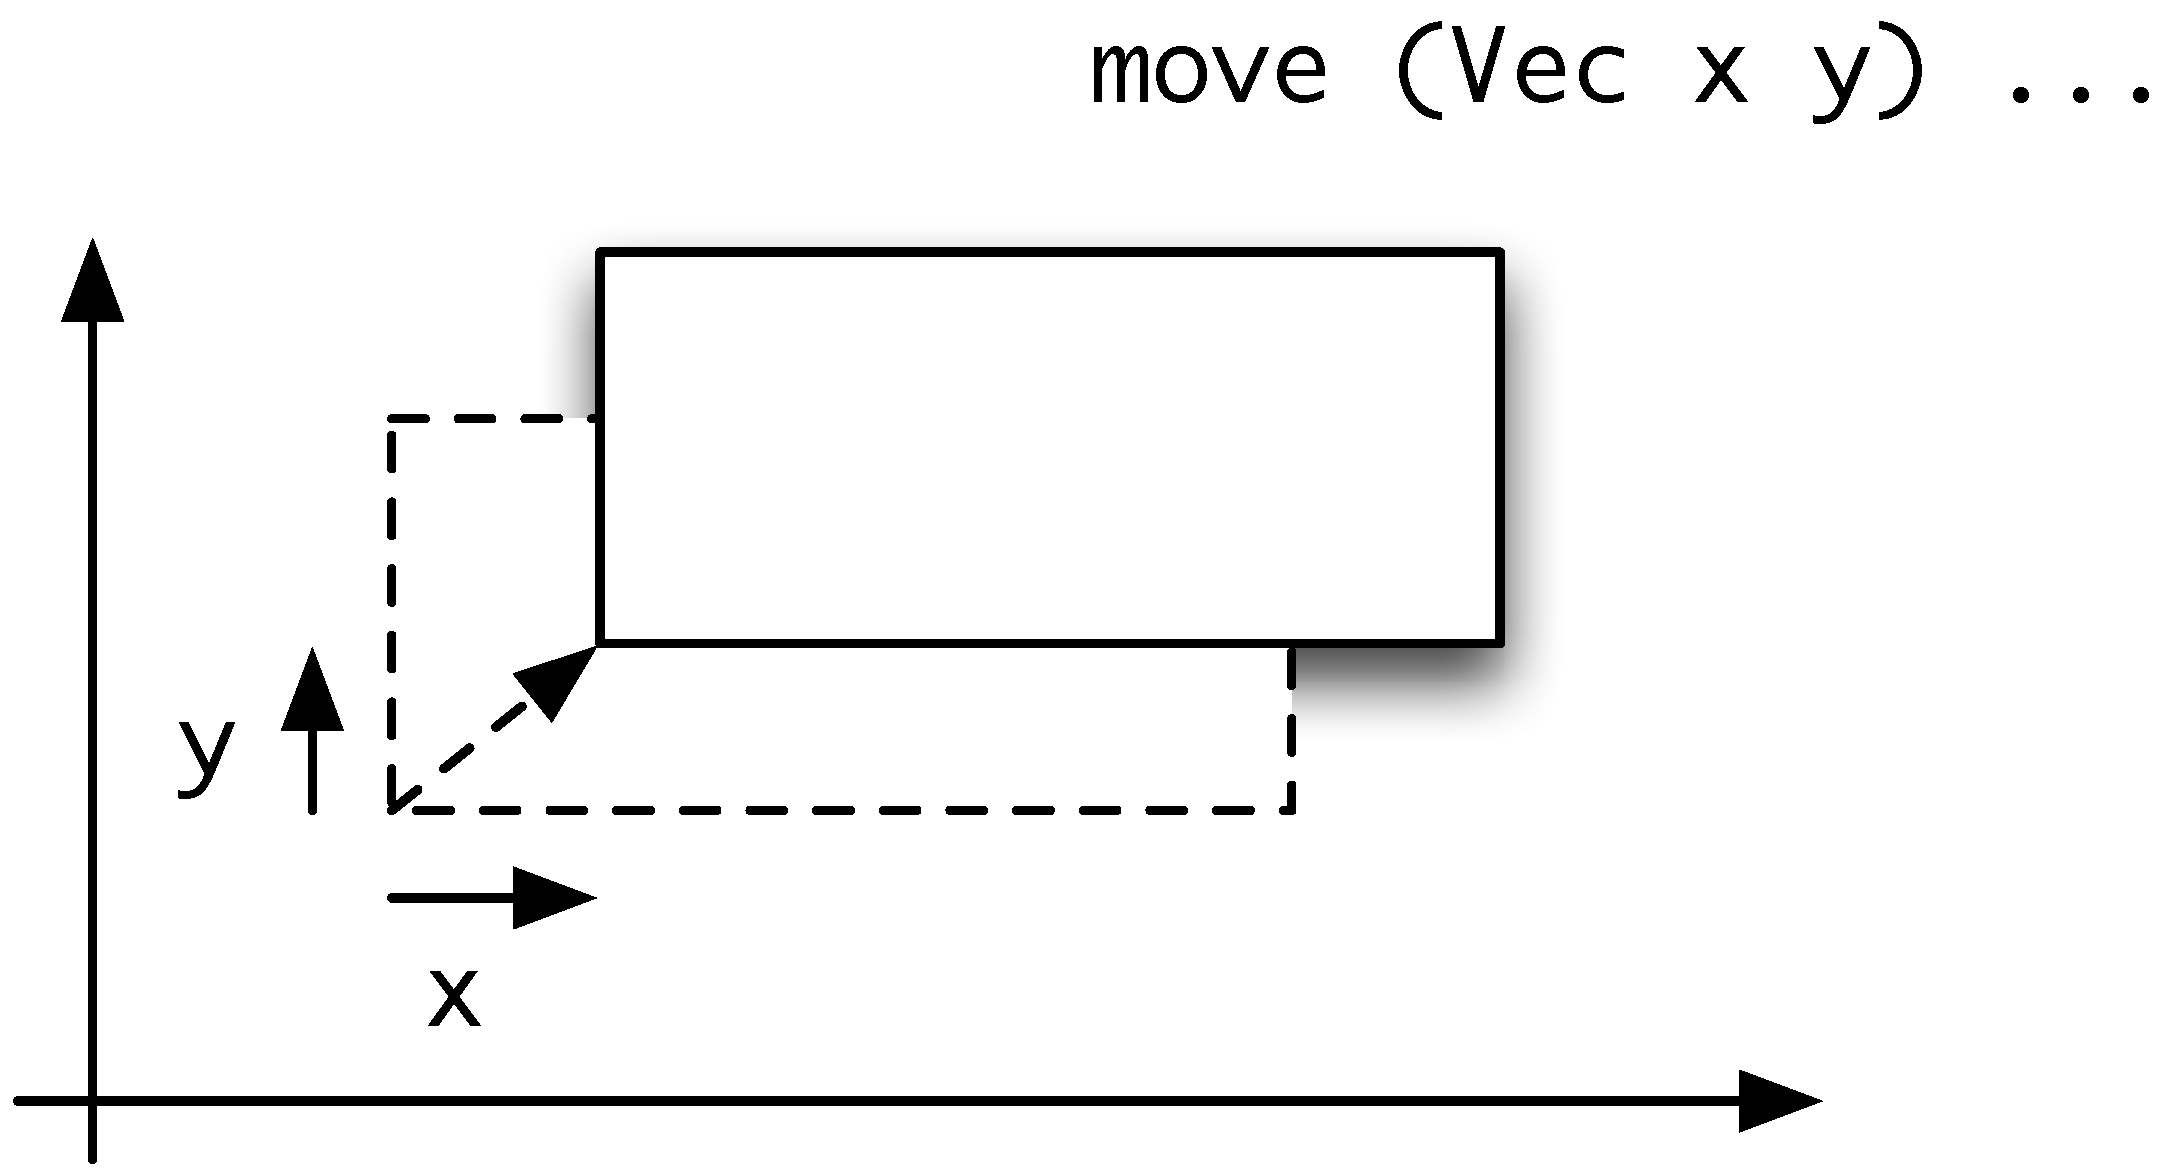
\includegraphics[width=3in]{Pictures/moveVec.pdf}
\end{center}

\begin{figure}[t]
\begin{alltt}
data Name a = Pair a String

exam1 = Pair (Point 0.0 0.0) "Dweezil"

instance Named (Name a) where\hfill(1)
  lookName (Pair obj nm) = nm
  giveName nm (Pair obj _) = (Pair obj nm)

mapName :: (a -> b) -> Name a -> Name b

mapName f (Pair obj nm) = Pair (f obj) nm

instance Movable a => Movable (Name a) where\hfill(2)
  move v   = mapName (move v)
  reflectX = mapName reflectX
  reflectY = mapName reflectY

class (Movable b, Named b) => NamedMovable b\hfill(3)\minx{NamedMovable}

instance Movable a => NamedMovable (Name a)
\end{alltt}
\caption{Named movable objects.}
\label{nMovObj}
\vspace{5pt}
\end{figure}



We can also reflect an object in the x-axis (the horizontal axis) or the y-axis
(the vertical),
or rotate a figure through $180^{\circ}$ around the origin (the point where
the axes meet). The default definition
of \texttt{rotate180} works by reflecting first in the y-axis and then
the x, as we did with the \texttt{Picture} type in Chapter \ref{intro}.


We can now define a hierarchy of movable objects; first we have the 
\texttt{Point},
\begin{alltt}
data Point = Point Float Float
             deriving Show
\end{alltt}
To make \texttt{Point} an instance of \texttt{Movable} we have to give
definitions of \texttt{move}, \texttt{reflectX} and \texttt{reflectY}
over the \texttt{Point} type.
\begin{alltt}
move (Vec v1 v2) (Point c1 c2) = Point (c1+v1) (c2+v2)
\end{alltt}
Here we can see that the move is achieved by adding the components \texttt{v1}
and \texttt{v2} to the coordinates of the point.
Reflection is given by changing the sign of one of the coordinates
\begin{alltt}
reflectX (Point c1 c2) = Point c1 (-c2)
reflectY (Point c1 c2) = Point (-c1) c2
\end{alltt}
For this instance we\index{classes!overriding defaults}
override the default definition of \texttt{rotate180} by changing the sign
of both coordinates. This is a more efficient way of achieving the same
transformation than the default definition.
\begin{alltt}
rotate180 (Point c1 c2) = Point (-c1) (-c2)
\end{alltt}
Using the type of points we can build figures:
\begin{alltt}
data Figure = Line Point Point |
              Circle Point Float
\end{alltt}
and in the instance declaration of \texttt{Movable} for \texttt{Figure} given in Figure
\ref{movOb2} we use the corresponding
operations on \texttt{Point}; for example,
\begin{alltt}
move v (Line p1 p2) = Line (move v p1) (move v p2)
move v (Circle p r) = Circle (move v p) r       
\end{alltt}
This same approach works again when we consider a list of movable objects:
\begin{alltt}
instance Movable a => Movable [a] where
  move v   = map (move v)
  reflectX = map reflectX
\end{alltt}
and so on. Using overloading in this way has a number of advantages.
\begin{titemize}
\item The code is much easier to read: at each point we write \texttt{move},
rather than \texttt{movePoint}, and so on.
\item We can reuse definitions; the instance declaration for 
\texttt{Movable [a]} makes lists of any sort of movable object movable themselves.
This includes lists of
points and lists of figures. Without overloading we would not be able to
achieve this.
\end{titemize}\index{overloading!advantages of}

\subsection*{Named objects}

Many forms of data contain some sort of name, a \texttt{String} which identifies
the object in question. What do we expect to be able to do with a value of
such a type?
\begin{itemize}
\item We should be able to identify the name of a value, and
\item we ought to be able to give a new name to a value.
\end{itemize}
These operations are embodied in the \texttt{Named} class:
\begin{alltt}
class Named a where\minx{Named}
  lookName :: a -> String
  giveName :: String -> a -> a
\end{alltt}
and an example of \texttt{Named} types is given by
\begin{alltt}
data Name a = Pair a String\minx{Name}
\end{alltt}
the one-constructor type whose two components are of type \texttt{a} and 
\texttt{String}. The \texttt{instance} declaration for this type is
\begin{alltt}
instance Named (Name a) where\hfill(1)
  lookName (Pair obj nm) = nm
  giveName nm (Pair obj _) = (Pair obj nm)
\end{alltt}

\subsection*{Putting together classes}
\index{classes!putting together}

An important aspect of object-oriented software development is the way in
which one class can be built upon another, reusing the operations of the
original class on the subclass. In this section we explore how to combine the
\texttt{Movable} and \texttt{Named} classes, to give objects which are both movable
and named. The section is
rather more advanced, and
can be omitted on first reading.


Suppose we are to add names to our movable objects -- how might this be done?
We examine one approach in the text, and another in the exercises.

Our approach is to build the type \texttt{Name a} where elements of type \texttt{a}
are movable, that is \texttt{Movable a} holds. We then
want to establish that the type \texttt{Name a} is in both the classes 
\texttt{Movable} and \texttt{Named}. We have shown the latter for {\em any\/} type 
\texttt{a} already in \texttt{(1)} above, so we concentrate on the former.


The crucial insight is that the naming is independent of the named type; any
operation on the type can be \textbf{lifted} to work over named types thus:
\begin{alltt}\minx{mapName}
mapName :: (a -> b) -> Name a -> Name b

mapName f (Pair obj nm) = Pair (f obj) nm
\end{alltt}
We can then argue that all the operations of the \texttt{Movable} class can be
lifted.
\begin{alltt}
instance Movable a => Movable (Name a) where\hfill(2)
  move v   = mapName (move v)
  reflectX = mapName reflectX
  reflectY = mapName reflectY
\end{alltt}
Now we already know that \texttt{Named (Name a)} by \texttt{(1)} above, so
if we define a class combining these attributes
\begin{alltt}
class (Movable b, Named b) => NamedMovable b\hfill(3)
\end{alltt}
we can declare the instance
\begin{alltt}
instance Movable a => NamedMovable (Name a)
\end{alltt}
This last instance is established by showing that the two constraints of
\texttt{(3)} hold when \texttt{b} is replaced by \texttt{Name a},
but this is exactly what \texttt{(1)} and \texttt{(2)} say given the constraint 
\texttt{Movable a}. 


This completes the demonstration that \texttt{NamedMovable (Name a)}
holds when we know that \texttt{Movable a}. It is worth realising that this demonstration is
produced automatically by the Haskell system -- we only need to type what is
seen in Figure \ref{nMovObj}.

This section has begun to illustrate how classes can be used in the software
development process. In particular we have shown how our movable objects can
be named in a way which allows reuse of all the code to move the objects.
\index{reuse}

\index{classes!and algebraic types|)}


\vspace{8pt}

\begin{exercises}
\vspace{3pt}

\item
A different way of combining the classes \texttt{Named} and \texttt{Movable} is to
establish the instance
\begin{alltt}
instance (Movable b,Named c) => NamedMovable (b,c)
\end{alltt}
This is done by giving the instances
\begin{alltt}
instance Movable b => Movable (b,c) where ....
instance Named c   => Named (b,c) where ....
\end{alltt}
Complete these instance declarations.

\item 
Show that the method of the previous question can be used to combine
instances of {\em any\/} two classes.

\item
The example in the final part of this section shows how we can combine an
arbitrary instance of the \texttt{Movable} class, \texttt{a},
with a {\em particular\/}
instance of the \texttt{Named} class, \texttt{String}. Show how it can be used to
combine an arbitrary instance of one class with a particular instance of
another for {\em any\/} two classes whatever.

\item
Extend the collection of operations for moving objects to include scaling and
rotation by an arbitrary angle. This can be done by re-defining \texttt{Movable}
or by defining a class \texttt{MovablePlus} over the class \texttt{Movable}. Which
approach is preferable? Explain your answer.

\item
Design a collection of classes to model bank accounts. These have different
forms: current, deposit and so on, as well as different levels of
functionality. Can you reuse the \texttt{Named} class here?
\end{exercises}

\section{Reasoning about algebraic types}
\index{proof!algebraic types}
\index{algebraic type!proofs}
%\label{algProofs}
\label{proofAlgTypes}

Verification for algebraic types follows the example of lists, as first
discussed in Chapter \ref{reasoningProgs}. The general pattern of structural
induction over an algebraic type states that the result has to be proved for
each constructor; when a constructor is recursive, we are allowed to use the
corresponding induction hypotheses in making the proof. We first give some
representative examples in this section, and conclude with a rather more
sophisticated proof.

\subsection*{Trees}
\minx{Tree}

Structural induction over the type \texttt{Tree}
of trees is stated as follows.
\subsubsection*{Structural induction over trees} 
\index{structural induction!trees}

To prove the property \texttt{P(tr)} for all finite \texttt{tr} of type 
\texttt{Tree t} we have to do two things.

\medskip
\noindent
\begin{mytable}
\bf \texttt{Nil} case & Prove \texttt{P(Nil)}. \\
\bf \texttt{Node} case & Prove \texttt{P(Node x tr1 tr2)} for all
\texttt{x} of
type \texttt{t}\\
& assuming that \texttt{P(tr1)} and 
\texttt{P(tr2)} hold already.
\end{mytable}

\medskip
\noindent
The advice of Chapter \ref{reasoningProgs} about finding proofs can easily be carried over to
the situation here. 
Now we give a representative
example of a proof. We aim to prove for all finite trees \texttt{tr} that
\begin{alltt}\index{map@\texttt{map}}\minx{collapse}\minx{mapTree}
map f (collapse tr) = collapse (mapTree f tr)\hfill(map-collapse)
\end{alltt}
which states that if we map a function over a tree, and then collapse the
result we get the same result as collapsing before mapping over the list.
The functions we use are defined as follows
\begin{alltt}
map f []     = [] \hfill (map.1)\index{map@\texttt{map}}
map f (x:xs) = f x : map f xs \hfill (map.2)

mapTree f Nil = Nil\hfill (mapTree.1)\minx{mapTree}
mapTree f (Node x t1 t2)
  = Node (f x) (mapTree f t1) (mapTree f t2) \hfill (mapTree.2)

collapse Nil = []\hfill (collapse.1)\minx{collapse}
collapse (Node x t1 t2)
  = collapse t1 ++ [x] ++ collapse t2\hfill (collapse.2)
\end{alltt}

\subparagraph{Base} In the \texttt{Nil} case, we simplify each side, giving
\begin{alltt}
map f (collapse Nil)
  = map f [] \hfill {\rm by} (collapse.1)
  = [] \hfill  {\rm by} (map.1)

collapse (mapTree f Nil)
  = collapse Nil \hfill {\rm by} (mapTree.1)
  = [] \hfill {\rm by} (collapse.1)
\end{alltt}
This shows that the base case holds.

\subparagraph{Induction} 
In the \texttt{Node} case, we have to prove:
\begin{alltt}
map f (collapse (Node x tr1 tr2)) 
  = collapse (mapTree f (Node x tr1 tr2))\hfill(ind)
\end{alltt}
assuming the two induction hypotheses:
\begin{alltt}
map f (collapse tr1) = collapse (mapTree f tr1) \hfill (hyp.1)
map f (collapse tr2) = collapse (mapTree f tr2)\hfill (hyp.2)
\end{alltt}
Looking at \texttt{(ind)}, we can simplify the left-hand side thus
\begin{alltt}
map f (collapse (Node x tr1 tr2))
  = map f (collapse tr1 ++ [x] ++ collapse tr2)\hfill{\rm by} (collapse.2)
  = map f (collapse tr1) ++ [f x] ++ map f (collapse tr2)
       \hfill{\rm by} (map++)
  = collapse (mapTree f tr1) ++ [f x] ++ 
    collapse (mapTree f tr2)\hfill{\rm by} (hyp1,hyp2) 
\end{alltt}
The final step is given by the two induction hypotheses, that the result
holds for the two subtrees \texttt{tr1} and \texttt{tr2}. The result \texttt{(map++)} is the
theorem
\begin{alltt}
map g (ys++zs) = map g ys ++ map g zs \hfill (map++)
\end{alltt}
discussed in Chapter \ref{gen2}. Examining the right-hand side now, we have
\begin{alltt}
collapse (mapTree f (Node x tr1 tr2))
  = collapse (Node (f x) (mapTree f tr1) 
                         (mapTree f tr2))\hfill{\rm by} (mapTree.2)
  = collapse (mapTree f tr1) ++ [f x] ++ 
    collapse (mapTree f tr2)\hfill{\rm by} (collapse.2)
\end{alltt}
and this finishes the proof in the \texttt{Node} case. As this is the
second
of the two cases, the proof is complete. 
\blackbox

\subsection*{The \texttt{Maybe} type}
\index{error handling!error type}
\minx{Maybe}

Structural induction for the type \texttt{Maybe t} becomes proof by cases --
because the type is not recursive, in none of the cases is there an appeal to
an induction hypothesis. The rule is

\subsubsection*{Structural induction over the \texttt{Maybe} type} 
\index{structural induction!\texttt{Maybe} type}

To prove the property \texttt{P(x)} for all defined\footnote{When the type is
not recursive, the induction principle gives a proof for all defined objects.
An object of this type is defined if it is \texttt{Nothing}, or \texttt{Just y} for a
defined \texttt{y}.}  \texttt{x} of type \texttt{Maybe t} we have to do two things:

\medskip
\noindent
\begin{mytable}
\bf \texttt{Nothing} case & Prove \texttt{P(Nothing)}. \\
\bf \texttt{Just} case & Prove \texttt{P(Just y)} for all defined \texttt{y} of type \texttt{t}.
\end{mytable}

\medskip
\noindent
Our example proof is that, for all defined values \texttt{x} of type 
\texttt{Maybe Int},
\begin{alltt}
maybe 2 abs x \(\geq\) 0\minx{maybe}
\end{alltt}

\startpr\ The proof has two cases. In the first \texttt{x} is replaced by 
\texttt{Nothing}:
\begin{alltt}
maybe 2 abs Nothing
  = 2 \(\geq\) 0
\end{alltt}
In the second, \texttt{x} is replaced by \texttt{Just y} for a defined \texttt{y}.
\begin{alltt}
maybe 2 abs (Just y)
  = abs y \(\geq\) 0
\end{alltt}
In both cases the result holds, and so the result is valid in general.
\blackbox

\subsection*{Other forms of proof}
\index{proof!non-primitive recursive}

We have seen that not all functions are defined by primitive recursion. The
example we saw in Section \ref{recTypes} was of the function \texttt{assoc},
which is used to rearrange arithmetic expressions represented by the type \texttt{Expr}. 
Recall that
\begin{alltt}
assoc (Add (Add e1 e2) e3)\minx{assoc}
  = assoc (Add e1 (Add e2 e3)) \hfill (assoc.1)
assoc (Add e1 e2) = Add (assoc e1) (assoc e2)\hfill (assoc.2)
assoc (Sub e1 e2) = Sub (assoc e1) (assoc e2)\hfill (assoc.3)
assoc (Lit n)     = Lit n\hfill (assoc.4)
\end{alltt}
with \texttt{(assoc.1)} being the non-primitive recursive case. We would like to
prove that the rearrangement does not affect the value of the expression:
\begin{alltt}\minx{eval}
eval (assoc ex) = eval ex \hfill (eval-assoc)
\end{alltt}
for all finite expressions \texttt{ex}. The induction principle for the \texttt{Expr}
\index{structural induction!expression type}
type has three cases.

\medskip
\noindent
\begin{mytable}
\bf \texttt{Lit} case & Prove \texttt{P(Lit n)}. \\
\bf \texttt{Add} case & Prove \texttt{P(Add e1 e2)}, assuming \texttt{P(e1)} and 
\texttt{P(e2)} \\
\bf \texttt{Sub} case & Prove \texttt{P(Sub e1 e2)}, assuming \texttt{P(e1)} and 
\texttt{P(e2)}
\end{mytable}

\medskip
\noindent
To prove \texttt{(eval-assoc)} for all finite expressions, we have the three cases given
above. The \texttt{Lit} and \texttt{Sub} cases are given, respectively, by 
\texttt{(assoc.4)} and \texttt{(assoc.3)}, but the \texttt{Add} case is more subtle. 
For this we will
prove
\begin{alltt}
eval (assoc (Add e1 e2)) = eval (Add e1 e2) \hfill (eval-Add)
\end{alltt}
by induction on the number of \texttt{Add}s which are left-nested at the top
level of the expression \texttt{e1} -- recall that it was by counting these
and noting that \texttt{assoc} preserves the total number of \texttt{Adds} overall
that we proved the function would always terminate. Now, if there are no 
\texttt{Add}s at the top-level of \texttt{e1}, the equation \texttt{(assoc.2)} gives \texttt{(eval-Add)}.
Otherwise we rearrange thus:
\begin{alltt}
eval (assoc (Add (Add f1 f2) e2))) 
= eval (assoc (Add f1 (Add f2 e2)))\hfill {\rm by} (assoc.1) 
\end{alltt}
and since \texttt{f1} contains fewer \texttt{Add}s at top level, 
\begin{alltt}
= eval (Add f1 (Add f2 e2))
= eval (Add (Add f1 f2) e2) \hfill {\rm by associativity of} +
\end{alltt}
which gives the induction step, and therefore completes the proof. 
\blackbox

This result shows that verification is possible for functions defined in a
more general way than primitive recursion.

\begin{figure}[t]\index{QuickCheck!properties of trees}
\beware{Checking properties in QuickCheck}{
Many of these properties can be checked in QuickCheck; we can define properties like this:
\begin{alltt}
prop\_assoc :: Expr -> Bool

prop\_assoc expr = 

\ \ \ \ eval expr == eval (assoc expr)

\ 

prop\_depth :: NTree -> Bool

prop\_depth t =

\ \ \ \ size t < 2\^{}(depth t)

\ 
    
prop\_collapse :: Eq b => (a -> b) -> Tree a -> Bool

prop\_collapse f =

\ \ \ \ \bs{t} -> map f (collapse t) == collapse (mapTree f t)
\end{alltt}
To be checkable, we need to be able to generate random values of the types \texttt{Expr}, \texttt{NTree} and \texttt{Tree a} (for types \texttt{a} for which random values can be generated). We have done this in the module available online, and we will explain the code in more detail in Chapter \ref{dsls}.
}
\end{figure}



\begin{exercises}

\item
Prove that the function \texttt{weather}\minx{weather} from Section \ref{introAlg} has the same
behaviour as  
\begin{alltt}
newWeather = makeHot . isSummer
\end{alltt}
when
\begin{alltt}
makeHot True  = Hot
makeHot False = Cold
isSummer = (==Summer)
\end{alltt}
where recall that \texttt{(==Summer)} is an operator section whose effect is to
test whether its argument is equal to \texttt{Summer}.

\item
Is it the case that the \texttt{area} of each \texttt{Shape} from Section
\ref{introAlg} is non-negative? If so, give a proof; if not, give an example
which shows that it is not the case.

\item
If we define the \texttt{size} of an \texttt{NTree} thus
\begin{alltt}
size NilT           = 0
size (Node x t1 t2) = 1 + size t1 + size t2
\end{alltt}
then prove that for all finite \texttt{nTree}s, \texttt{tr},
\begin{alltt}
size tr \(<\) \(\mbox{\texttt{2}}^{\mbox{\texttt{(depth tr)}}}\)
\end{alltt}

\item
Show for all finite \texttt{NTree}s \texttt{tr} that
\begin{alltt}
occurs tr x = length (filter (==x) (collapse tr))
\end{alltt}

\medskip
\noindent
The next two exercises refer back to the exercises of Section \ref{polyAlg}.

\item
Prove that the function \texttt{twist} has the property that
\begin{alltt}
twist . twist = id
\end{alltt}

\item
Explain the principle of structural induction for the type \texttt{GTree}.
Formulate and prove the equivalent of the theorem relating \texttt{map}, 
\texttt{mapTree} and \texttt{collapse} for this type of trees.
\end{exercises}
\begin{summary}
Algebraic types sharpen our ability to model types in our programs: we have
seen in this chapter how simple, finite types like \texttt{Temp} can be defined,
as well as the more complex \texttt{Either} and recursive types. Many of these
recursive types are varieties of tree\index{tree}: we looked at numerical trees; elements
of the type \texttt{Expr} can also be thought of as trees representing the
underlying structure of arithmetical 
expressions.

The type of lists gives a guiding example for various aspects of algebraic
types.
\begin{titemize}
\item The definition of the type is
recursive and polymorphic, and many polymorphic higher-order
functions can be defined over lists -- this carries over to the various types
of tree and the error type, \texttt{Maybe}, for example.
\item There is a simple
principle for reasoning over lists, structural induction, which is the model
for structural induction over algebraic types.
\end{titemize}
The chapter also gives guidelines for defining algebraic types. The definition
can be given in three parts: first the type name is identified, then the
constructors are named, and finally their component types are specified. As
in other aspects of program development, this separation of concerns assists
the system developer to produce simple and correct solutions.

Having introduced algebraic data types we are able to give more substantial
examples of classes and their instances. We can see that the overloading that
classes bring makes code both easier to read and more amenable to reuse; we can see in
particular how software can be extended in a way that requires little
modification to the code.

In the chapters to come, algebraic types will be an integral part of the
systems we develop, and indeed in the next case study we exhibit various
aspects of these types. We shall also explore a different approach to types:
abstract data types, and see how this approach complements and contrasts with
the use of algebraic data types.

\index{algebraic type|)}

\end{summary}



%\end{document}
